% LaTeX Article Template - using defaults
\documentclass[9pt,twoside]{exam}
%\textheight    23cm
%\textwidth     17.cm
%\oddsidemargin   .1cm
%\evensidemargin  .1cm
%\topmargin -0.9cm
%\parskip 3pt
%\pagestyle{myheadings}

\usepackage[english]{babel}
\usepackage{graphicx}
%\usepackage{showkeys}
\usepackage{datetime}
\usepackage[applemac]{inputenc}
\usepackage{amssymb,amsmath}
\usepackage[T1]{fontenc}
\usepackage{caption}
\usepackage{subcaption}
\usepackage{hyperref}
\usepackage{graphicx}
\usepackage[absolute]{textpos}
\usepackage{anyfontsize}
\usepackage{t1enc}
\usepackage[usenames, dvipsnames]{color}
\usepackage{lipsum}
\usepackage{tcolorbox}
\usepackage{float}


% A nice serif font, but no the prescribed nonfree ITC stone
\usepackage[oldstylenums]{kpfonts}
\usepackage[T1]{fontenc}
%\usepackage{fancyhdr}
\definecolor{mygray1}{RGB}{128, 128, 128}
\definecolor{mygray2}{RGB}{77, 77, 77}
% No paragraph indentation
\pagestyle{empty}
\newcommand{\bigbar}{\rule[0ex]{0.41pt}{.75in}} 

\newcommand{\R}{\ensuremath{\mathbb R}}


\begin{document}
%%%%%%%%%%%%%%%%%%%%%%%%%%%%%%%%%%%%%%%%%%%
%%%%%%%%%%%%%%%%%%%%%%%%%%%%%%%%%%%%%%%%%%%
%%%%                       COVER PAGE begins                         %%%%%%%%%%%%%
%%%%%%%%%%%%%%%%%%%%%%%%%%%%%%%%%%%%%%%%%%%
%%%%%%%%%%%%%%%%%%%%%%%%%%%%%%%%%%%%%%%%%%%
%\begin{coverpages}
\title{\begin{tcolorbox} \begin{center}{CS 470\\ 
\vspace{0.5cm}
Data Mining\\
\vspace{0.5cm}
Homework 1\\
 } \end{center}
 \end{tcolorbox}}
% \vspace{2cm}
 \author{ 
 Jason Ji \\\\
Collaborations: Richard Yang, https://plotly.com/python/, \\https://pandas.pydata.org/docs/reference/api/pandas.DataFrame.html}
 \date{  }
 \maketitle
\pagestyle{myheadings}
\thispagestyle{plain}
\markboth{\; \hrulefill\;Homework 1 -  CS 470}{\; Homework 1 -  CS 470 \hrulefill\; }
\vspace{-0.5cm}



%%%%%%%%%%%%%%%%%%%%%%%%%%%%%%%%%%%%%%%%%%%
%%%%%%%%%%%%%%%%%%%%%%%%%%%%%%%%%%%%%%%%%%%
%%%%                       COVER PAGE ends                            %%%%%%%%%%%%%
%%%%%%%%%%%%%%%%%%%%%%%%%%%%%%%%%%%%%%%%%%%
%%%%%%%%%%%%%%%%%%%%%%%%%%%%%%%%%%%%




\newcommand{\bi}{\mathbf{i}}
\newcommand{\bbb}{\mathbf{b}}



\section*{Problem 1 -  [Attribute description]}

Semester: ordinal data that describes which year and semester is it that the student took the CS 170 course. The attribute is ordinal because it has a meaningful order (F17, S17, F18, S18 ...).
\\\\
Student ID: categorical data that represents the unique identity of each student.
\\\\
Name: categorical data that represents the name of the student
\\\\
Section: categorical data that describe the class section that the student is in.
\\\\
Homework 1-5: numeric interval data (because there is no absolute 0 -- people will receive 20 points if they submit early, even if they get all the answers wrong) that represents the score one receives on each homework assignment.
\\\\
Peer evaluation: numeric ratio data (because one could receive a 0 score due if they don't do the peer evaluation) that measures how one contributes to evaluating others' code. However, if one still receives a score higher than 0 if they don't do the peer evaluation, this will be numeric interval data.
\\\\
Bonus: numeric ratio data (assuming one will receive a 0 score if they don't have any bonuses) that measures how many bonuses one receives by identifying typos.  
\\\\
Quiz 01-12: data that measures the score received by students on the quizzes. Depending on how the quiz is graded, it may or may not have an absolute zero. If there is absolute zero and the division of scores makes sense, then it is a numeric ratio. If students can get partial grades for completion even if they answer all the questions wrong, it is a numeric interval.
\\\\
Quiz Adjustment: numeric ratio data (assuming students receive 0 when there are no particular circumstances, which indicates the existence of absolute zero) that represents particular circumstances such as regraded quiz score, a make-up quiz, or an extra drop.
\\\\
Drop Lowest Quiz 1-2: numeric interval (because it falls below zero and division doesn't make sense) that represents the two lowest quiz scores that are subtracted from the total score.
\\\\
Final Exam:  data that represents the final exam score received by the students. Depending on how the final exam is graded, it may or may not have an absolute zero. If students still receive partial credit for completion even if they get all the answers wrong, there is no absolute zero and it is a numeric interval. However, if the division of scores makes sense and there is an absolute zero, then it is a numeric ratio. 
\\\\
Total Score: numeric ratio data (assuming if the student doesn't do anything in class and receives a 0 total score, there is an absolute zero) that represents the total score one receives in the entire semester. 
\\\\
Letter Grade: ordinal data (because there is a meaningful order and ranking) that represents the letter grade received by the student based on their total scores.
\\\\

\section*{Problem 2 -  [Missing values]}

There are missing values in all Homeworks, Peer Evaluations, Bonus, all Quizzes, both Quiz Adjustment, and Final Exam.\\

Homeworks:

Meanings: 
Missing value means the student didn't submit any homework for that specific homework assignment or submitted it very late.


Solutions:

Solution 1: replace the missing value with 0
Solution 2: replace the missing value with this specific homework's average score
Solution 3: replace the missing value with the average score of all homework of this student 


Pros and Cons:

Solution 1: punish the student for missing homework since it will bring down his grade. However, it seems to be the best approach because it reflects the grade student should have received. But it can't reflect the true difficulty of that particular homework.


Solution 2: useful if we are analyzing the homework difficulty and comparing the average scores of homeworks. In this case, the average homework score would have fewer outliers and can reflect the homework difficulty. However, it will affect student's final grade and make it very inaccurate.


Solution 3: this can be useful when a student is excused from that homework due to special circumstances. This reflects the true ability of the student. However, this will affect the final grade of the student and might be very unfair to the rest of the students.\\


Peer Evaluation

Meanings:

Missing values in Peer Evaluation means that the student either didn't give other peer evaluations or didn't receive enough peer evaluations 


Solutions:

Solution 1: replace the missing value with 0
Solution2: replace the missing value with the average peer evaluation score in that term 
Solution3: delete the entire peer review column


Pros and Cons:


Solution 1: punish the student for missing peer evaluation since it will bring down his grade, but it can't reflect the true ability of the student because maybe it's just his/her peers forgot to submit evaluations but this student is being punished.

Solution 2: Can reflect the difficulty of the peer review when analyzing peer evaluations across different terms. However, it will affect students' final grades and make them inaccurate.

Solution 3: this will remove all missing values along with all present values. However, it will make the final grade inaccurate because the peer evaluation is completely removed. \\


Bonus


Meanings:


Missing values mean that the student didn't get any bonus point


Solutions:


Solution 1: replace the missing value with 0
Solution 2: replace the missing value with the average of bonuses of all students in that class


Pros and Cons:


Solution 1: This seems to be the best solution because it accurately reflects the fact that this student didn't receive any bonus points. 

Solution 2: This will make the student's final grade inaccurate and the total bonus points received by all the students in that class inaccurate.\\ 



Quizzes

Meanings: 
Missing value means the student didn't do that quiz. 


Solutions:

Solution 1: replace the missing value with 0
Solution 2: replace the missing value with this specific quiz's average score
Solution 3: replace the missing value with the average score of all quizzes of this student 


Pros and Cons:

Solution 1: punish the student for missing the quiz since it will bring down his grade. However, it seems to be the best approach because it reflects the grade student should have received. But it can't reflect the true difficulty of that particular quiz.


Solution 2: useful if we are analyzing the quiz difficulty and comparing the average scores of quizzes. In this case, the average quiz score would have fewer outliers and can reflect the quiz difficulty. However, it will affect students' final grades and make them very inaccurate.


Solution 3: this can be useful when a student is excused from that quiz due to special circumstances (in addition to dropping the two lowest quizzes). This reflects the true ability of the student. However, this will affect the final grade of the student and might be very unfair to the rest of the students.\\


Quiz adjustments

Meaning: missing values mean the student didn't receive any regrade on their quizzes

Solution: replace the missing value with 0

Pros and cons: 
This solution seems to be very fair because it reflects the actual situation and doesn't affect any other values in the table. Also useful if we are comparing the average quiz adjustments across sections or terms. \\

Final Exam

Meaning: missing values mean the student didn't take the final exam

Solution: replace the missing value with 0

Pros and cons: 
This solution seems to be very fair because it reflects the actual situation and doesn't affect any other values in the table. Also useful if we are comparing the average final exam scores across sections or terms. 

\section*{Problem 3 -  [Re-encoding]}

The attributes Semester and Section are not encoded (represented) in a very smart way. For the semester, it doesn't specify which year it is which might cause a wrong interpretation. For example, people may think it is 1918 rather than 2018 looking at the value "F18". Instead, it should be represented in the following format: "Year + Season" like "2018Fall". In this way, if we want to order the student by the semester, it will correctly put them in the order of time. For the section, the only thing provided was the section number, which could be confusing and doesn't provide useful information by itself. A solution to this is to combine the semester and section information (ex. "2018Fall01"), which uniquely identifies which class belongs to which semester rather than only having a single-digit encoding. We can name this new column "Class". This also make it easy for ordering.\\
Please see the code.py and modified grades.csv files for the re-encoding in the data set.

\section*{Problem 4 -  [Scaling and z-scoring]}
All score-related attributes go through the same process shown below.\\
Please see the code.py and modified grades.csv files for rescaling details.\\
Take homework 1 as an example, the first student Youyang (student Id 457364) has a score of 32 for homework 1. 

1. Re-scaled to the interval [0,100]: \\
    Formula: $Z_{i} = (X_{i} - min(X)) / (max(X) - min(X)) \cdot 100$. \\
    $Score_{new} = (32 - 0)/(44-0) * 100 = 72.7$. 

2. z-scoring with mean and standard deviation from all semesters combined: \\
    Formula: $Z = (X - \mu) / \sigma$. \\
    $Score_{new} = (32 - 37.78)/7.25 = -0.8$. 

3. z-scoring with mean and standard deviation from only the students in their same semester:\\
    Formula: $Z = (X - \mu) / \sigma$. \\
    $Score_{new} = (32 - 37.82)/6.72 = -0.866$. 
\\

Analysis: for result 1, it simply re-scaled the score to a 100 score scale. It is useful if we want to see the percentage of its score out of the perfect score. However, it doesn't provide much insight into the student's performance relative to their peers. For result 2, it is the normalized score relative to the entire data set, meaning it represents the performance of the student on homework 1 compared to all other students in the data set. This method is appropriate if we want to compare this student with all the students who took homework 1 previously in this class, and the result shows the student scores slightly below the mean of all students. For result 3, it is the normalized score relative to the students in the same semester. This is useful if we want to only compare the student with their peers, students who took CS170 at the same time as them. In this example, the z score is similar to result 2, which means Youyang is performing slightly below the average performance of students who took this class at the same time.



\section*{Problem 5 -  [Summary statistics]}
\begin{center}
\begin{tabular}{ c c c c c c c c}
  & Mean & Standard Deviation & Min & Q1 & Median & Q3 & Max  \\ 
 Homework 1 &  37.784595 & 7.251365 &  0.0  & 37.00   &   40.0   &   42.000 &     44.0 \\  
 Homework 2 &  37.984355 & 6.332375 & 0.0   &   37.00 &     40.0 &     41.000  &    44.0 \\  
 Homework 3 &  37.470976 &  6.900583 & -7.0  &    36.00   &   40.0   &   42.000  &    44.0 \\  
 Homework 4 &  37.993369 &  6.747088 &  -3.0   &   37.00   &   40.0   &   42.000  &    44.0 \\  
 Homework 5 &  40.095816 &  6.363133 &0.0   &   40.00   &   42.0  &    42.000     & 44.0 \\  
 Peer Evaluations &  146.591263 & 16.185329 & 1.0  &   150.00  &   150.0   &  150.000 &    150.0 \\  
 Bonus &   2.266667 &  1.709915 &  1.0   &    1.00   &    1.0   &    3.500   &    5.0 \\  
 Quiz 01 &  38.649283 & 11.314150 &  5.0  &    30.00   &   43.0   &   49.000    &  50.0\\  
 Quiz 02 &   42.769129 &  9.911537 & 0.0   &   39.00   &   46.0   &   50.000   &   50.0 \\  
 Quiz 03 &   34.319426 &  10.799184 &  1.0  &    28.00  &    37.0  &    42.000  &    50.0\\  
 Quiz 04 &  41.817819 & 8.492970 &  0.0    &  39.00   &   45.0 &     48.000 &     50.0 \\  
 Quiz 05 &  36.634899 & 11.718397 & 0.0  &    30.00 &     40.0  &    46.000 &     50.0 \\  
 Quiz 06 &  34.118529 & 11.679011 &  2.0  &    26.00  &    37.0   &   43.000  &    50.0 \\  
 Quiz 07 &  34.383356 & 13.025263 & 0.0   &   25.00   &   37.0   &   46.000  &    50.0 \\ 
 Quiz 08 &   32.702446 & 14.190149 & 0.0   &   23.00  &    36.0    &  44.000  &    50.0 \\  
 Quiz 09 &  30.291156 & 12.334887 &  0.0   &   21.00  &    30.0   &   40.000  &    50.0 \\  
 Quiz 10 &  31.056088 & 11.495127 & 0.0  &    23.00 &     32.0  &    41.000 &     50.0 \\  
 Quiz 11 &   37.781740 & 14.849993 & 0.0  &    31.00    &  44.0   &   50.000  &    50.0
\\  
 Quiz 12 &  36.822695 & 15.340030 &0.0    &  28.00  &    43.0    &50.000  &    50.0\\  
 Quiz Adjustment &  34.620000 & 5.900621 & 25.5   &   30.20 &     35.2 &     37.675&      43.0\\  
 Drop Lowest Quiz 1 &  -14.279337 & 13.615211 &  -48.0   &  -26.00   &  -13.0 &      0.000   &    0.0 \\  
 Drop Lowest Quiz 2 &  -21.625638 & 13.773500 & -49.0   &  -32.25  &   -24.0     &-10.000    &   0.0 \\  
 Final Exam &   109.550471 & 21.071367 &  24.0  &    99.00 &    114.0  &   126.000  &   147.0 \\  
 Total Score &  798.954847 & 185.856883 & 0.0  &   738.75 &    852.5  &   926.000&    1000.0
\\  

\end{tabular}
\end{center}



\section*{Problem 6 -  [Charts]}
1. Homework 1 box plot \\
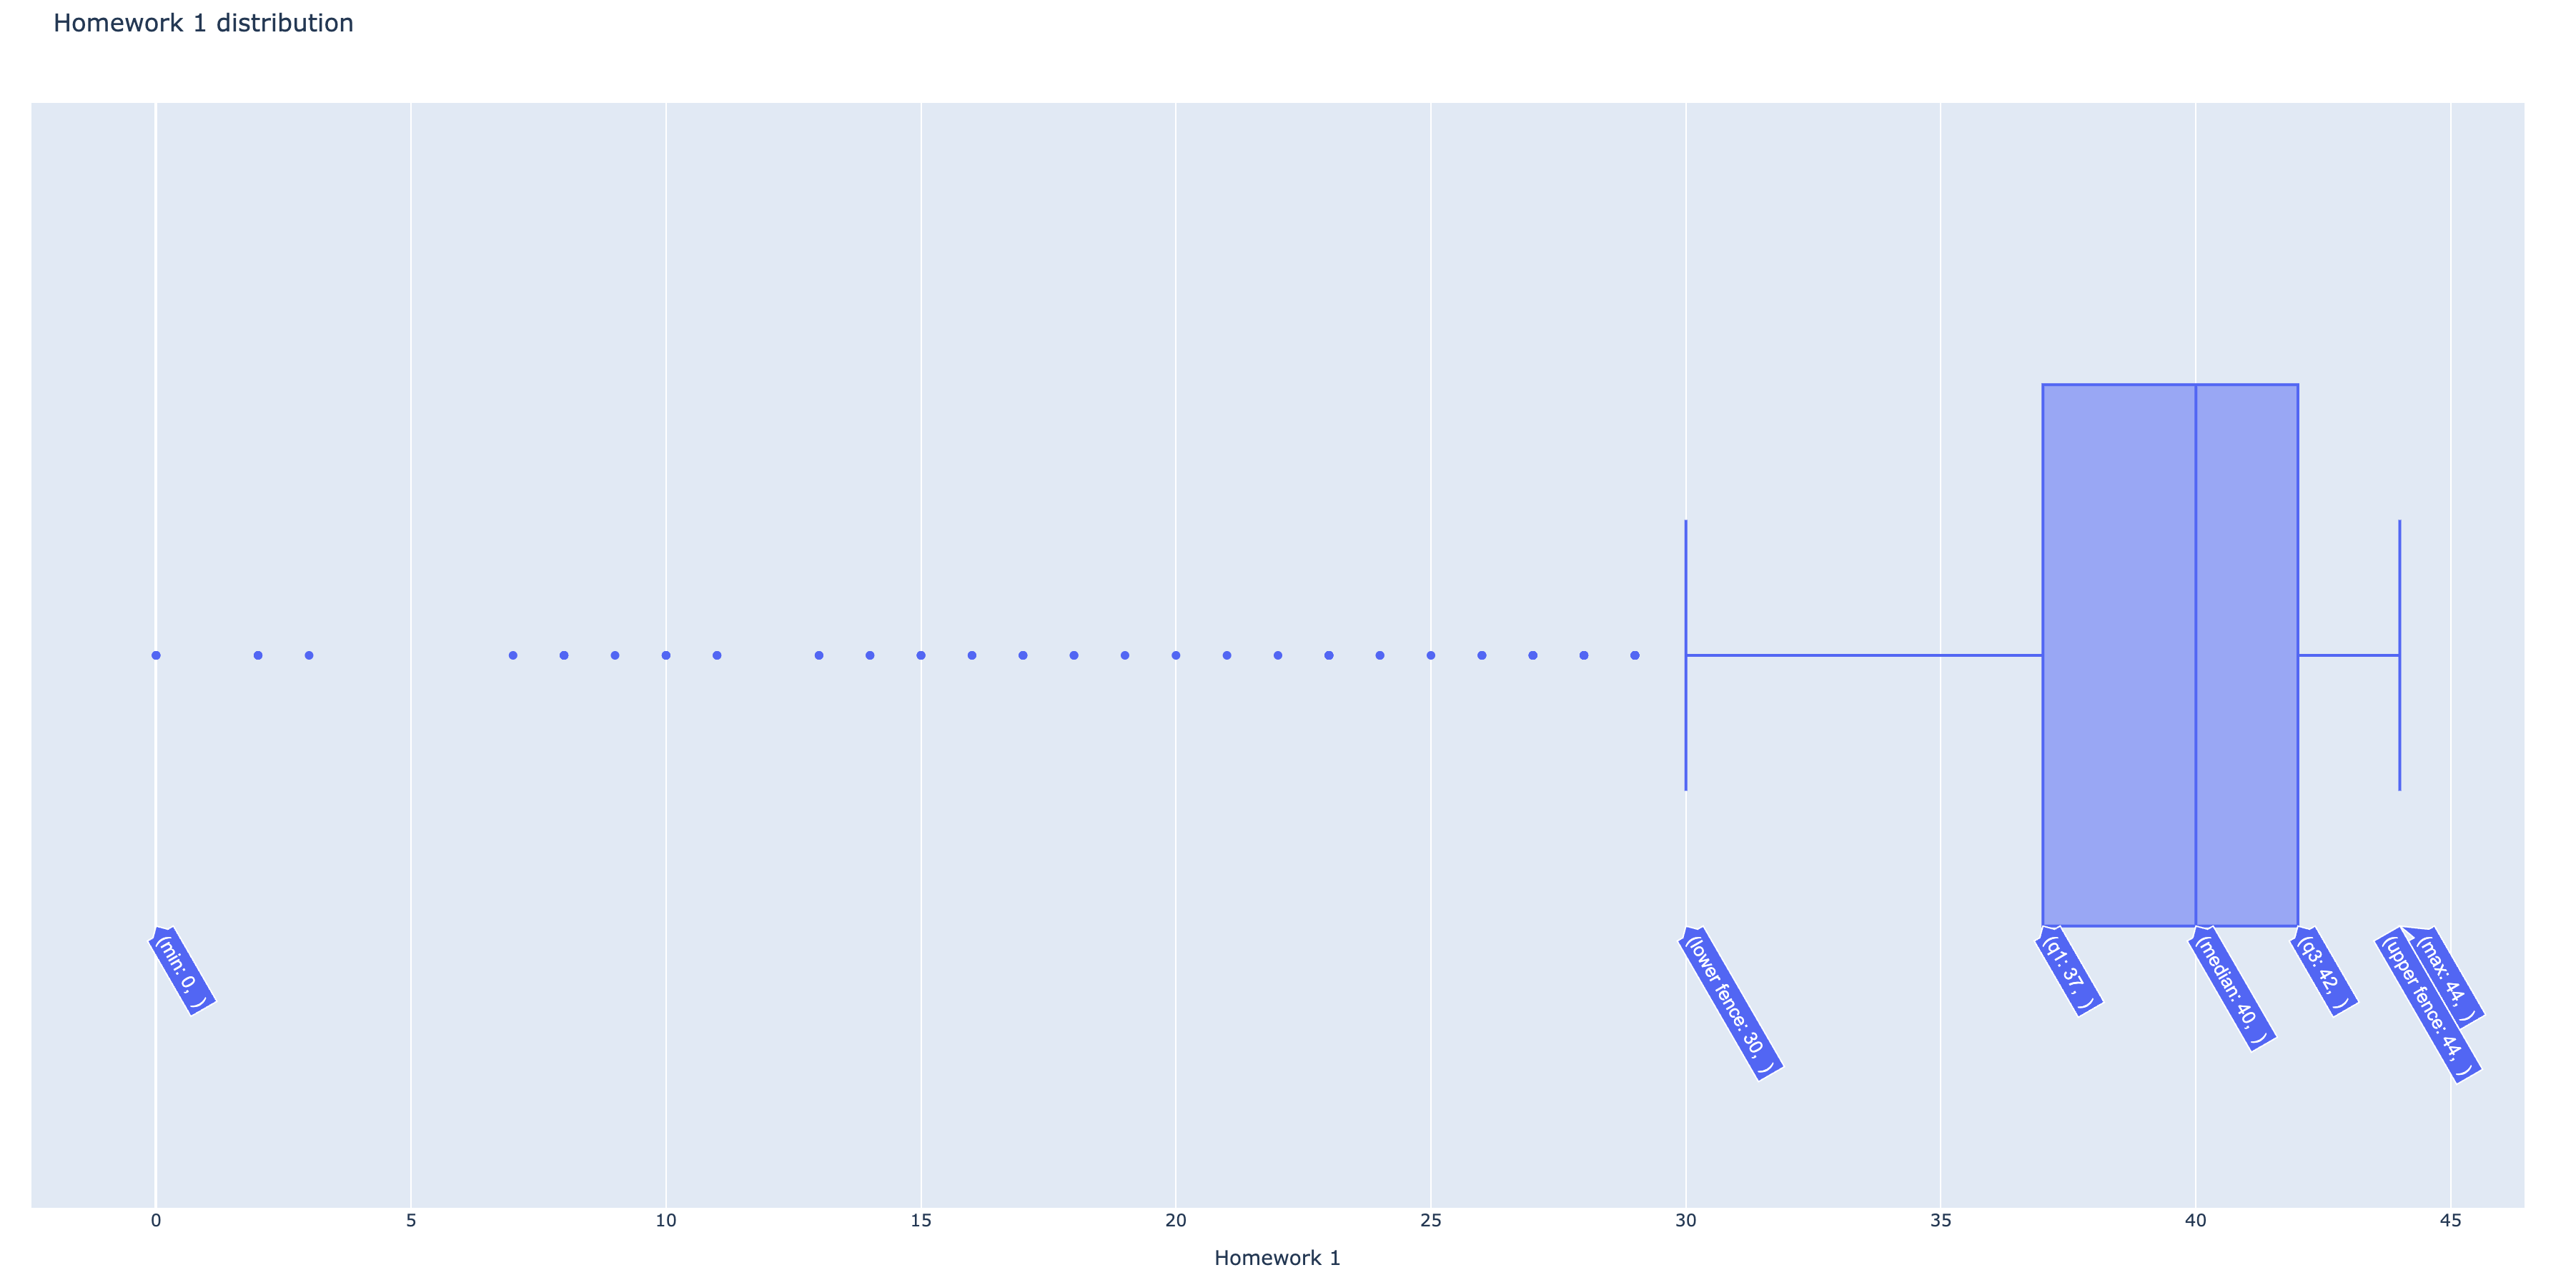
\includegraphics[width=15cm, height=8cm]{hw1.png}\\
This box plot shows the score distribution of all students who submitted homework 1. As we can see, the box plot shows the score range of homework 1 with a minimum of 0, a lower fence of 30, a q1 of 37, a median of 40, a q3 of 43, and an upper fence and a maximum of 44. One thing that is noticeable is that half of the students receive a full score or more than a full score. There are also a lot of outliers on the lower bound, representing students who receive low grades. \\\\
2. Homework 2 box plot \\
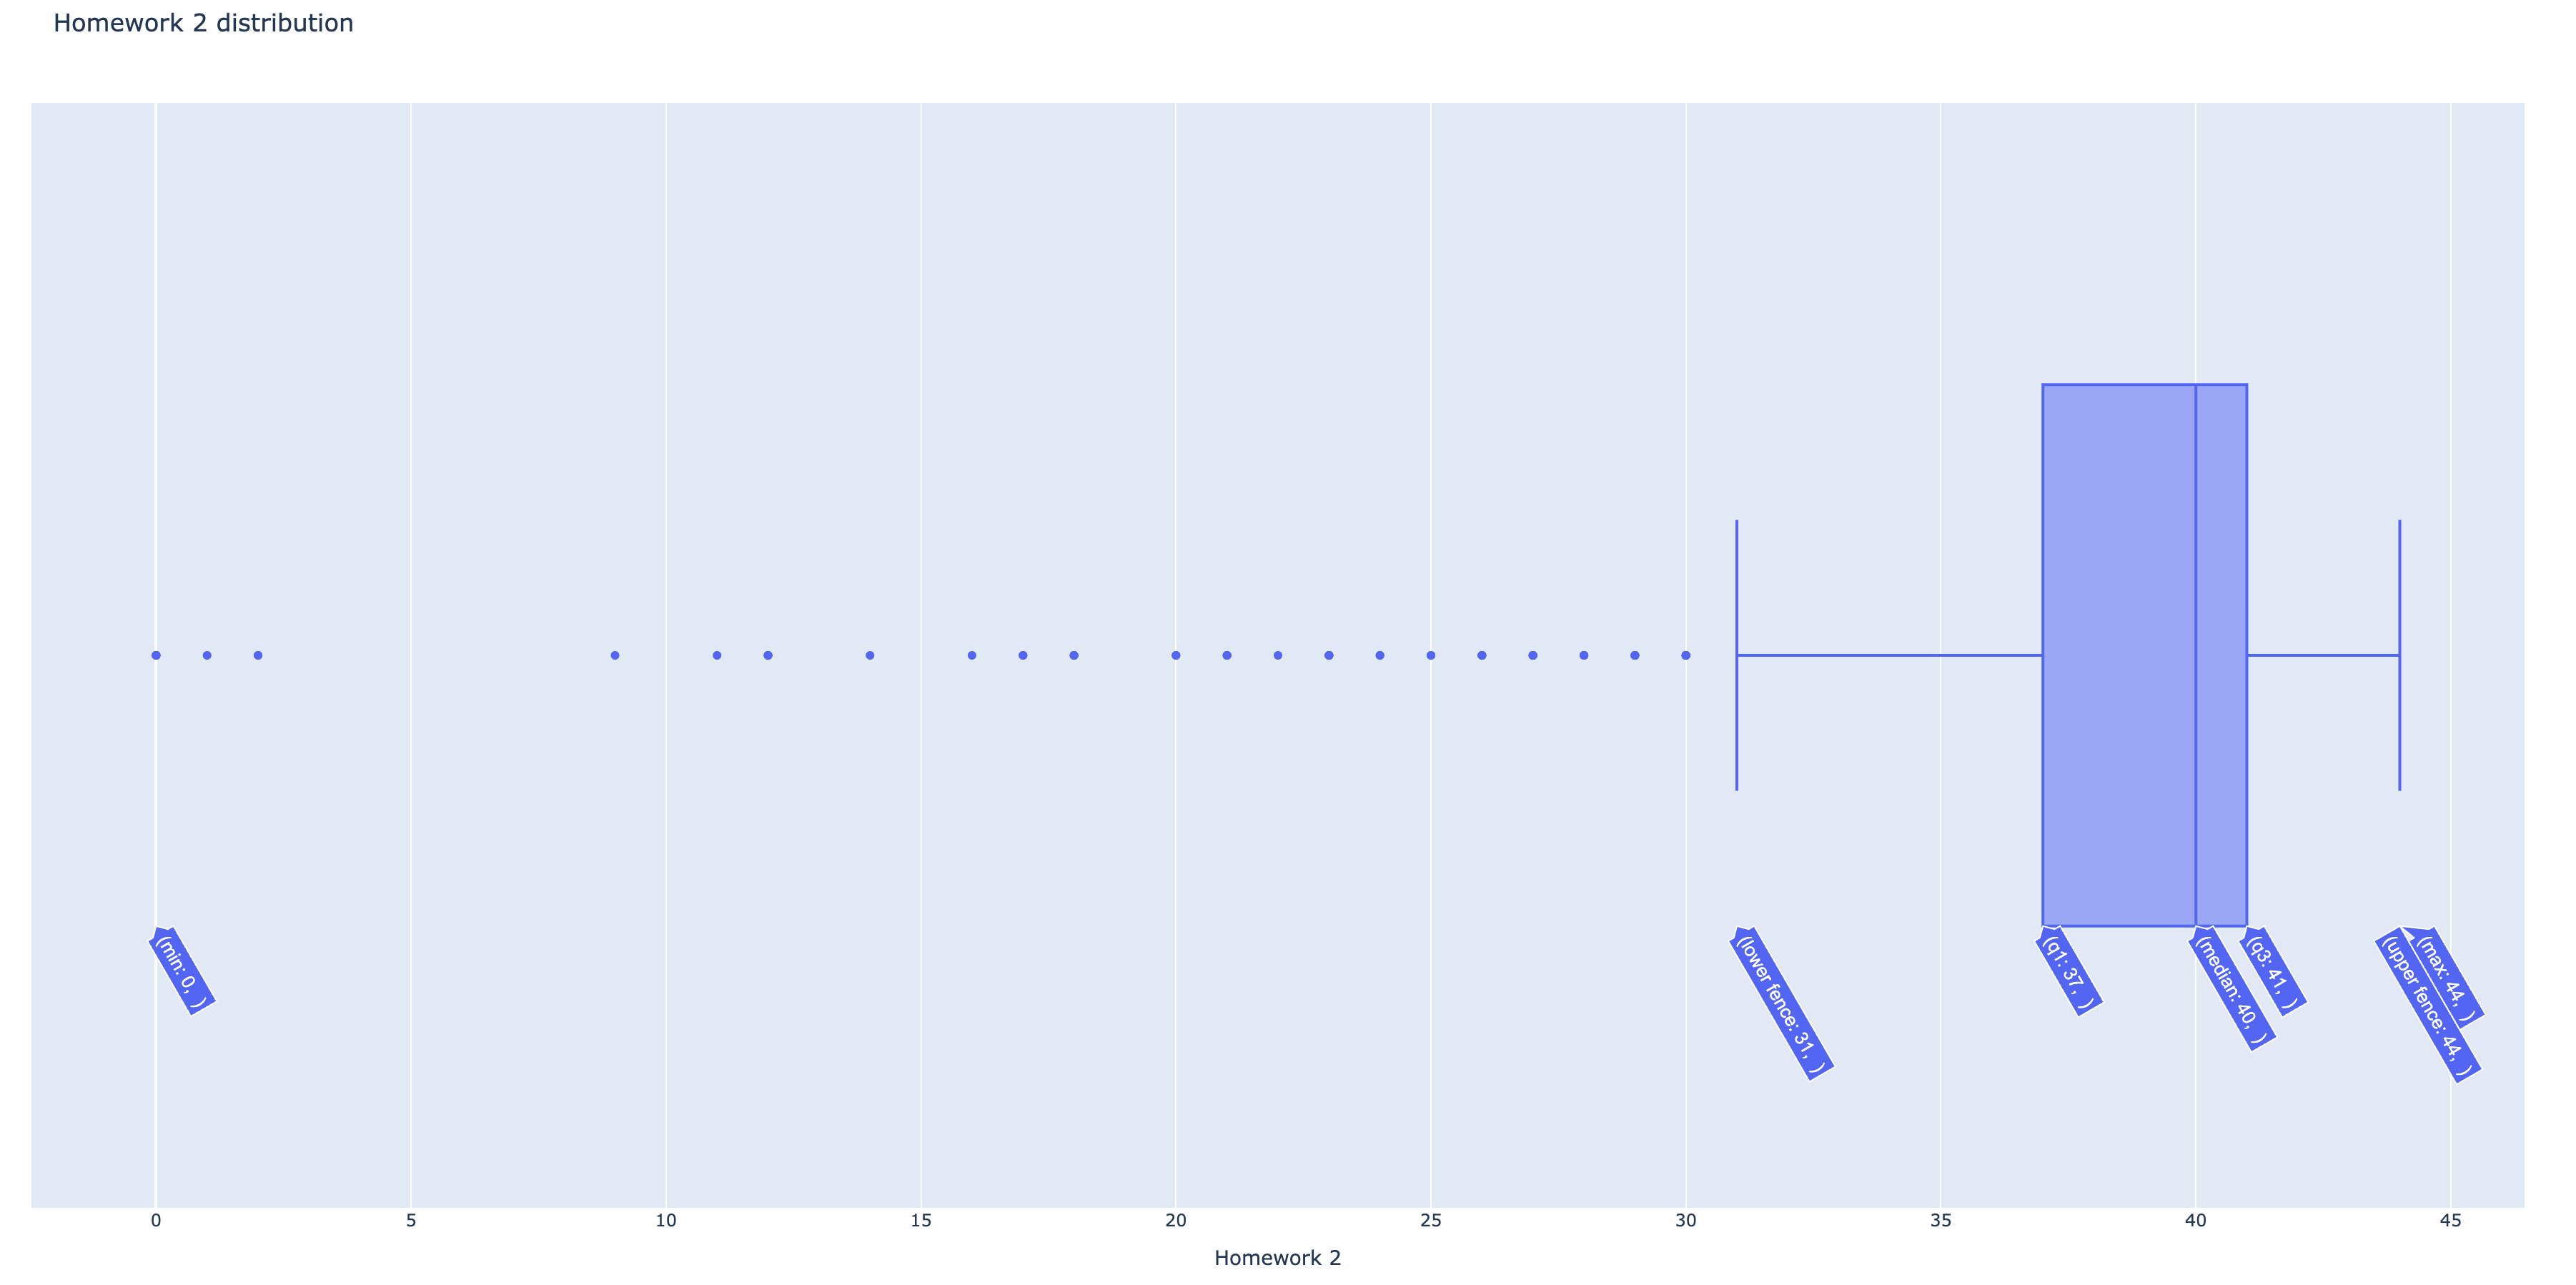
\includegraphics[width=15cm, height=8cm]{hw2.png}\\
This box plot shows the score distribution of all students who submitted homework 2. As we can see, the box plot shows the score range of homework 2 with a minimum of 0, a lower fence of 31, a q1 of 37, a median of 40, a q3 of 41, and an upper fence and a maximum of 44. One thing that is noticeable is that the homework 2 scores are more concentrated (has a lesser range) compared to homework 1. The q3 is 41, which is less than 43 -- the q3 for homework 1. \\\\
3. Homework 3 box plot \\
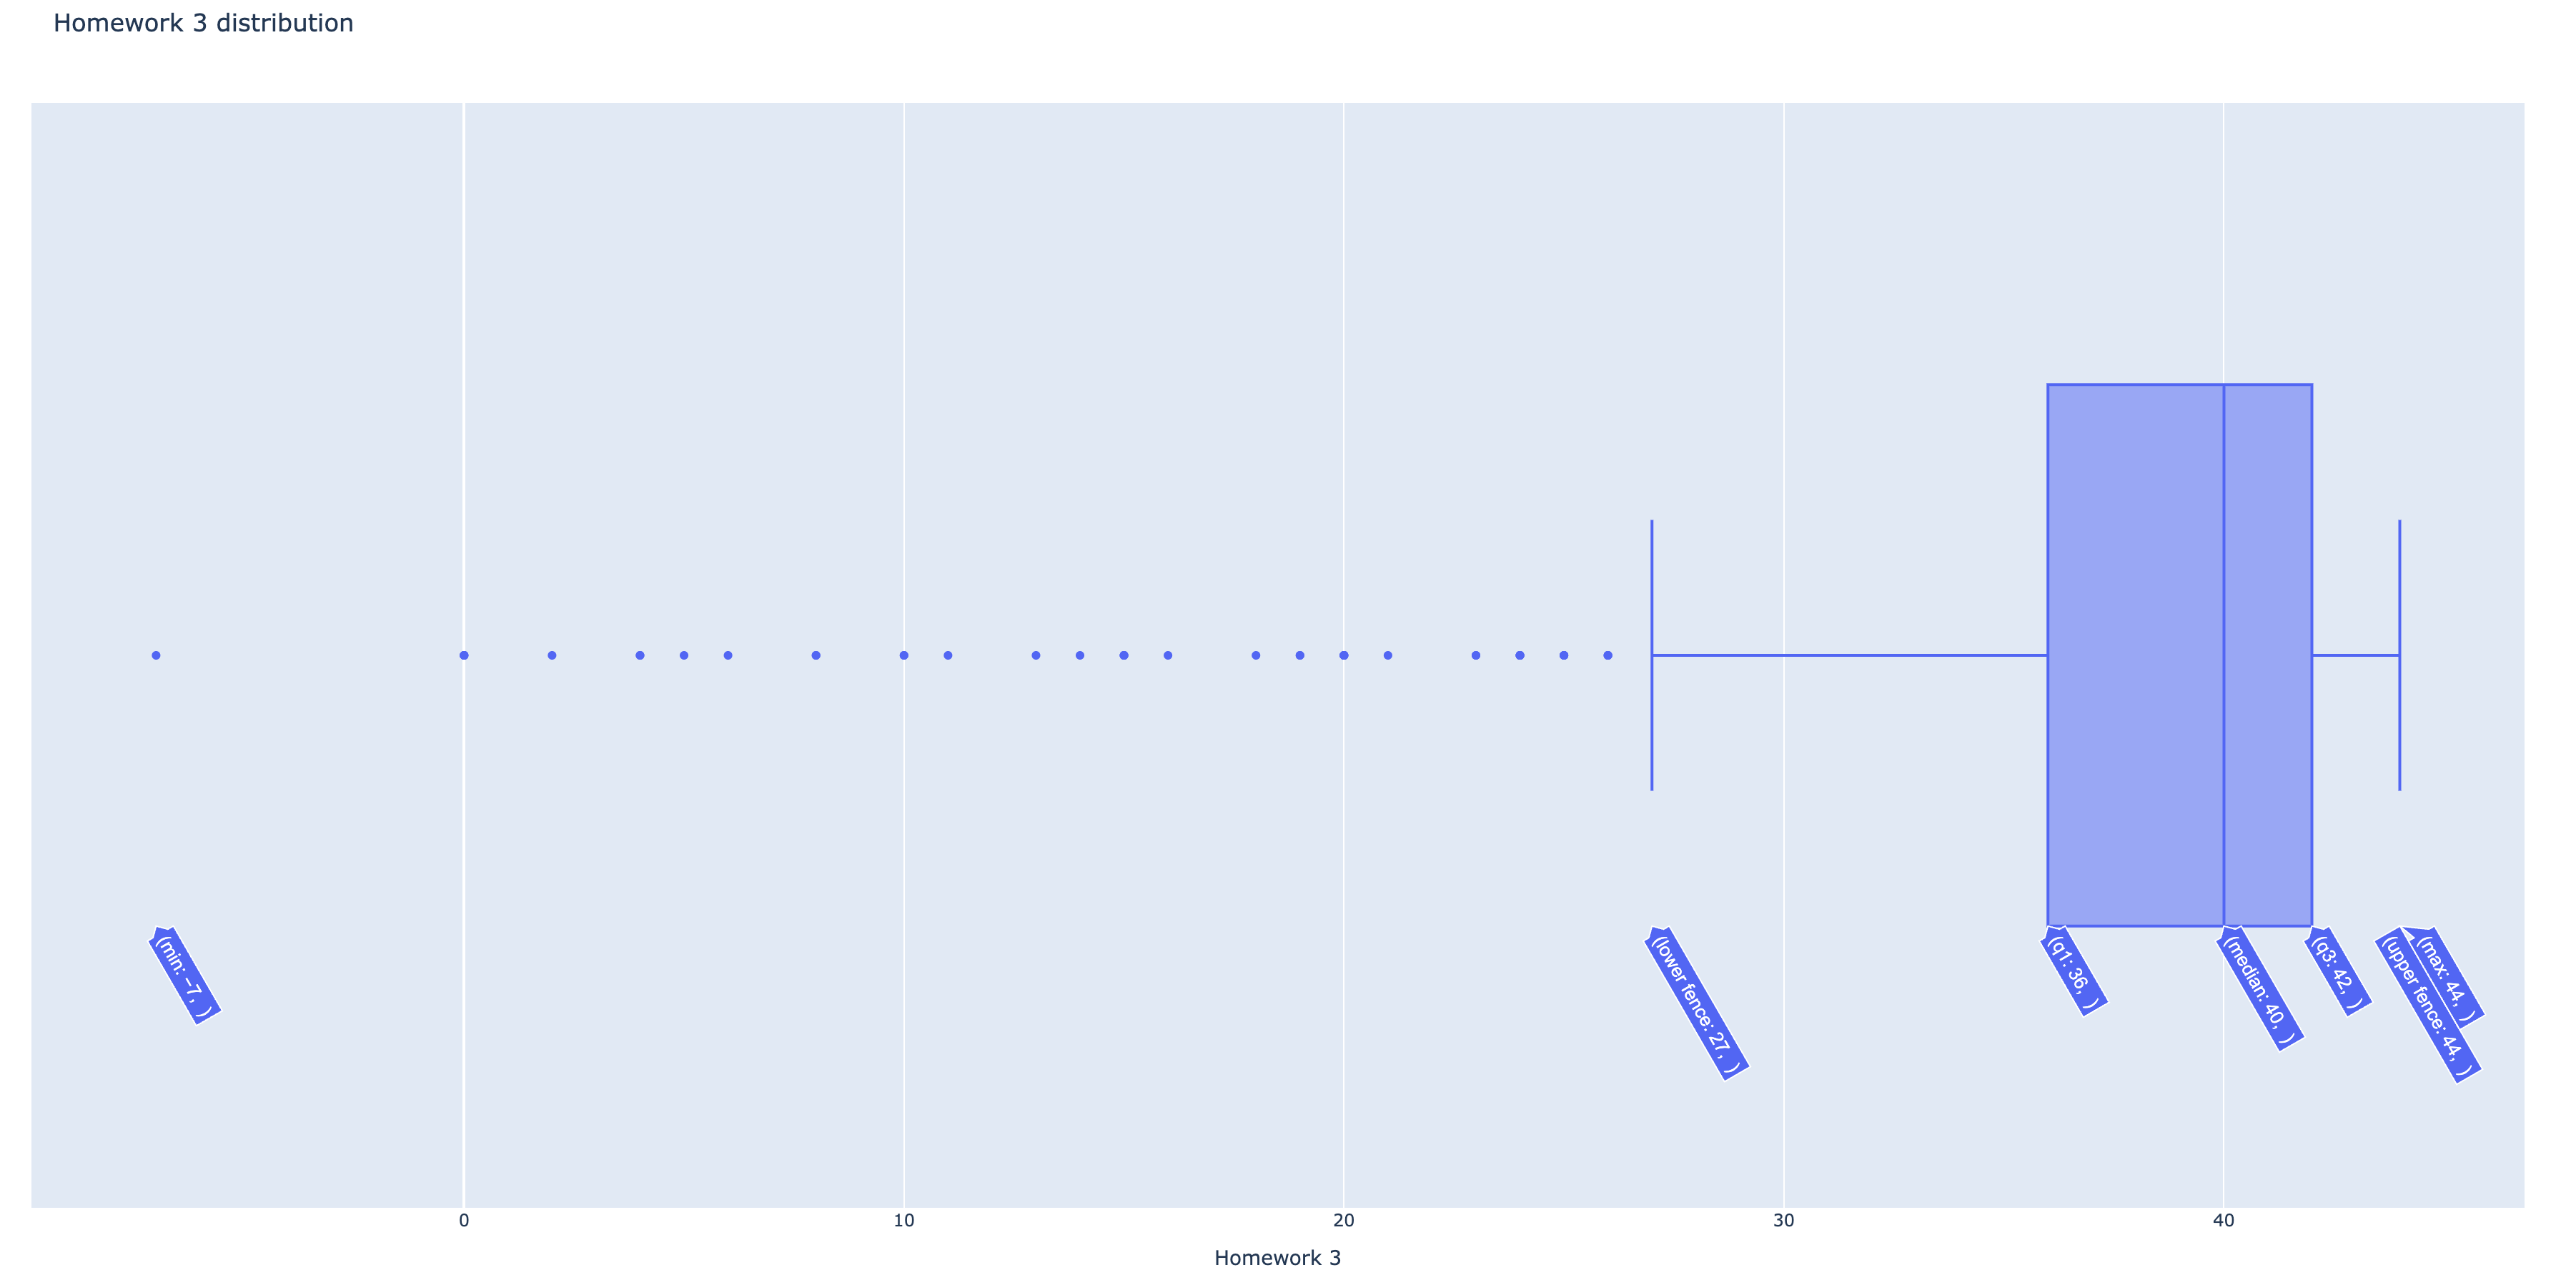
\includegraphics[width=15cm, height=8cm]{hw3.png}\\
This box plot shows the score distribution of all students who submitted homework 3. As we can see, the box plot shows the score range of homework 3 with a minimum of -7, a lower fence of 27, a q1 of 36, a median of 40, a q3 of 42, and an upper fence and a maximum of 44. One thing that is noticeable is that there are more lower scores in 
 homework 3 than in both homework 1 and 2. The lower fence is 27 and q1 is 36, which are both lower than the lower fences and q1 for homework 1 and 2. \\\\
4. Peer Evaluations histogram  \\
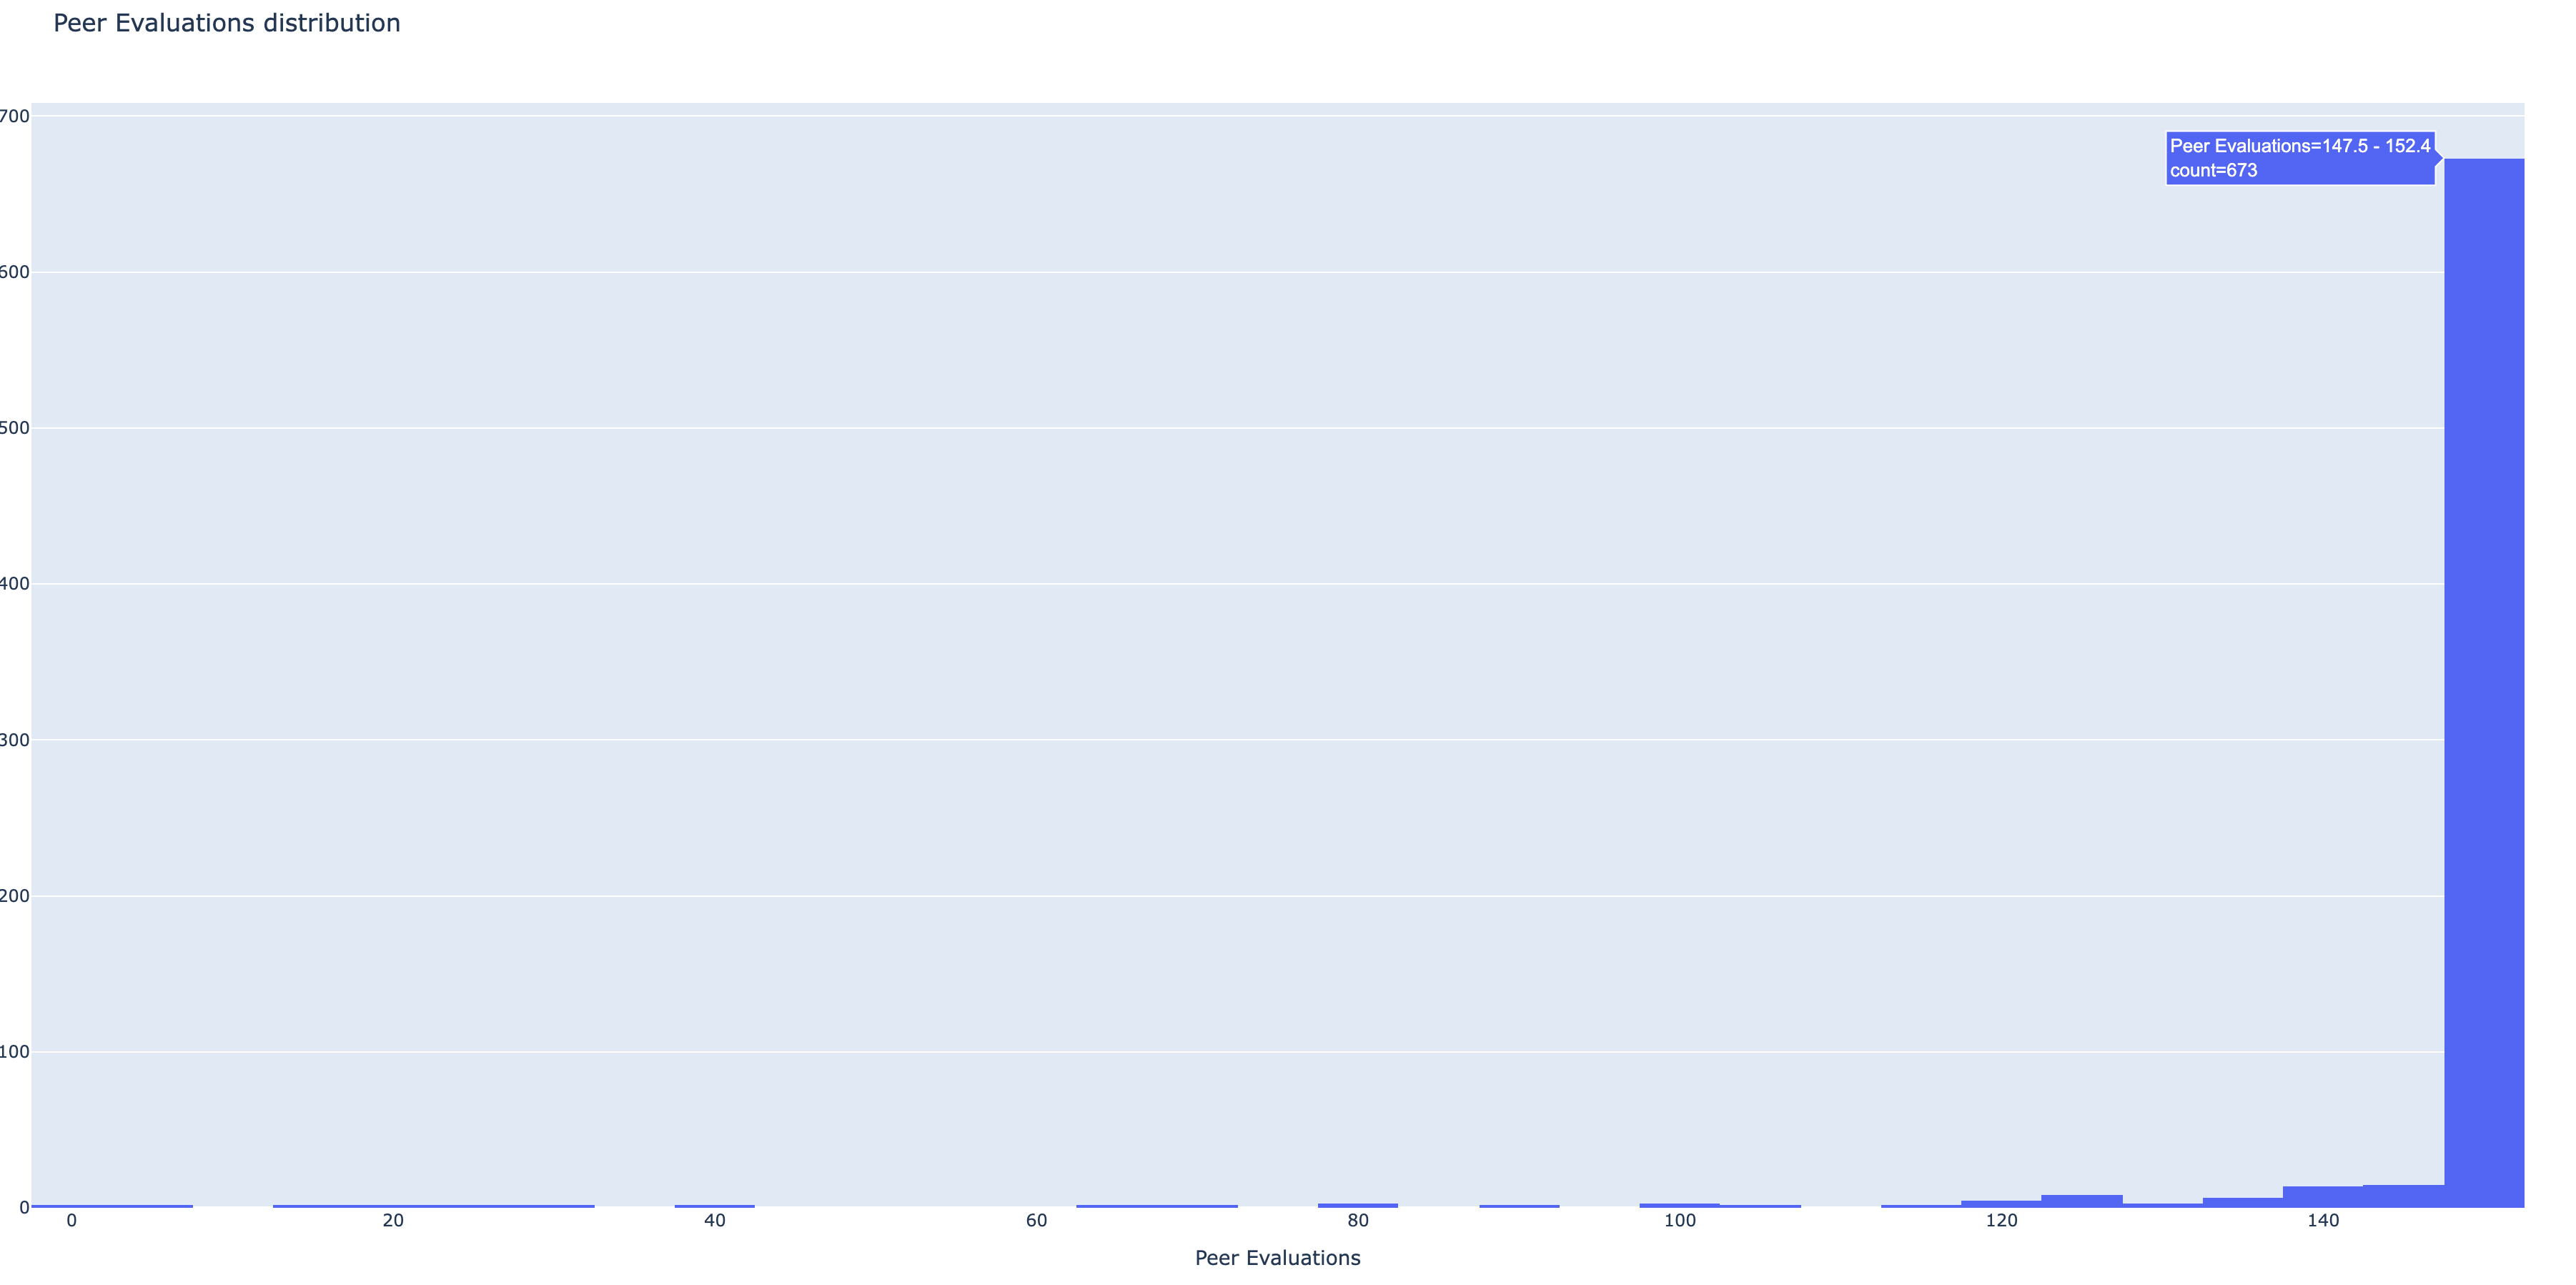
\includegraphics[width=15cm, height=8cm]{hist1.png}\\
This histogram shows the frequency distribution of the peer evaluations scores for all students. From the graph we can see that the mast majority of scores received by students is between the range 147.5 and 152.4, which has a count of 673. This means that almost all the students receive a full score on this assignment.\\\\
5. Final Exam histogram \\
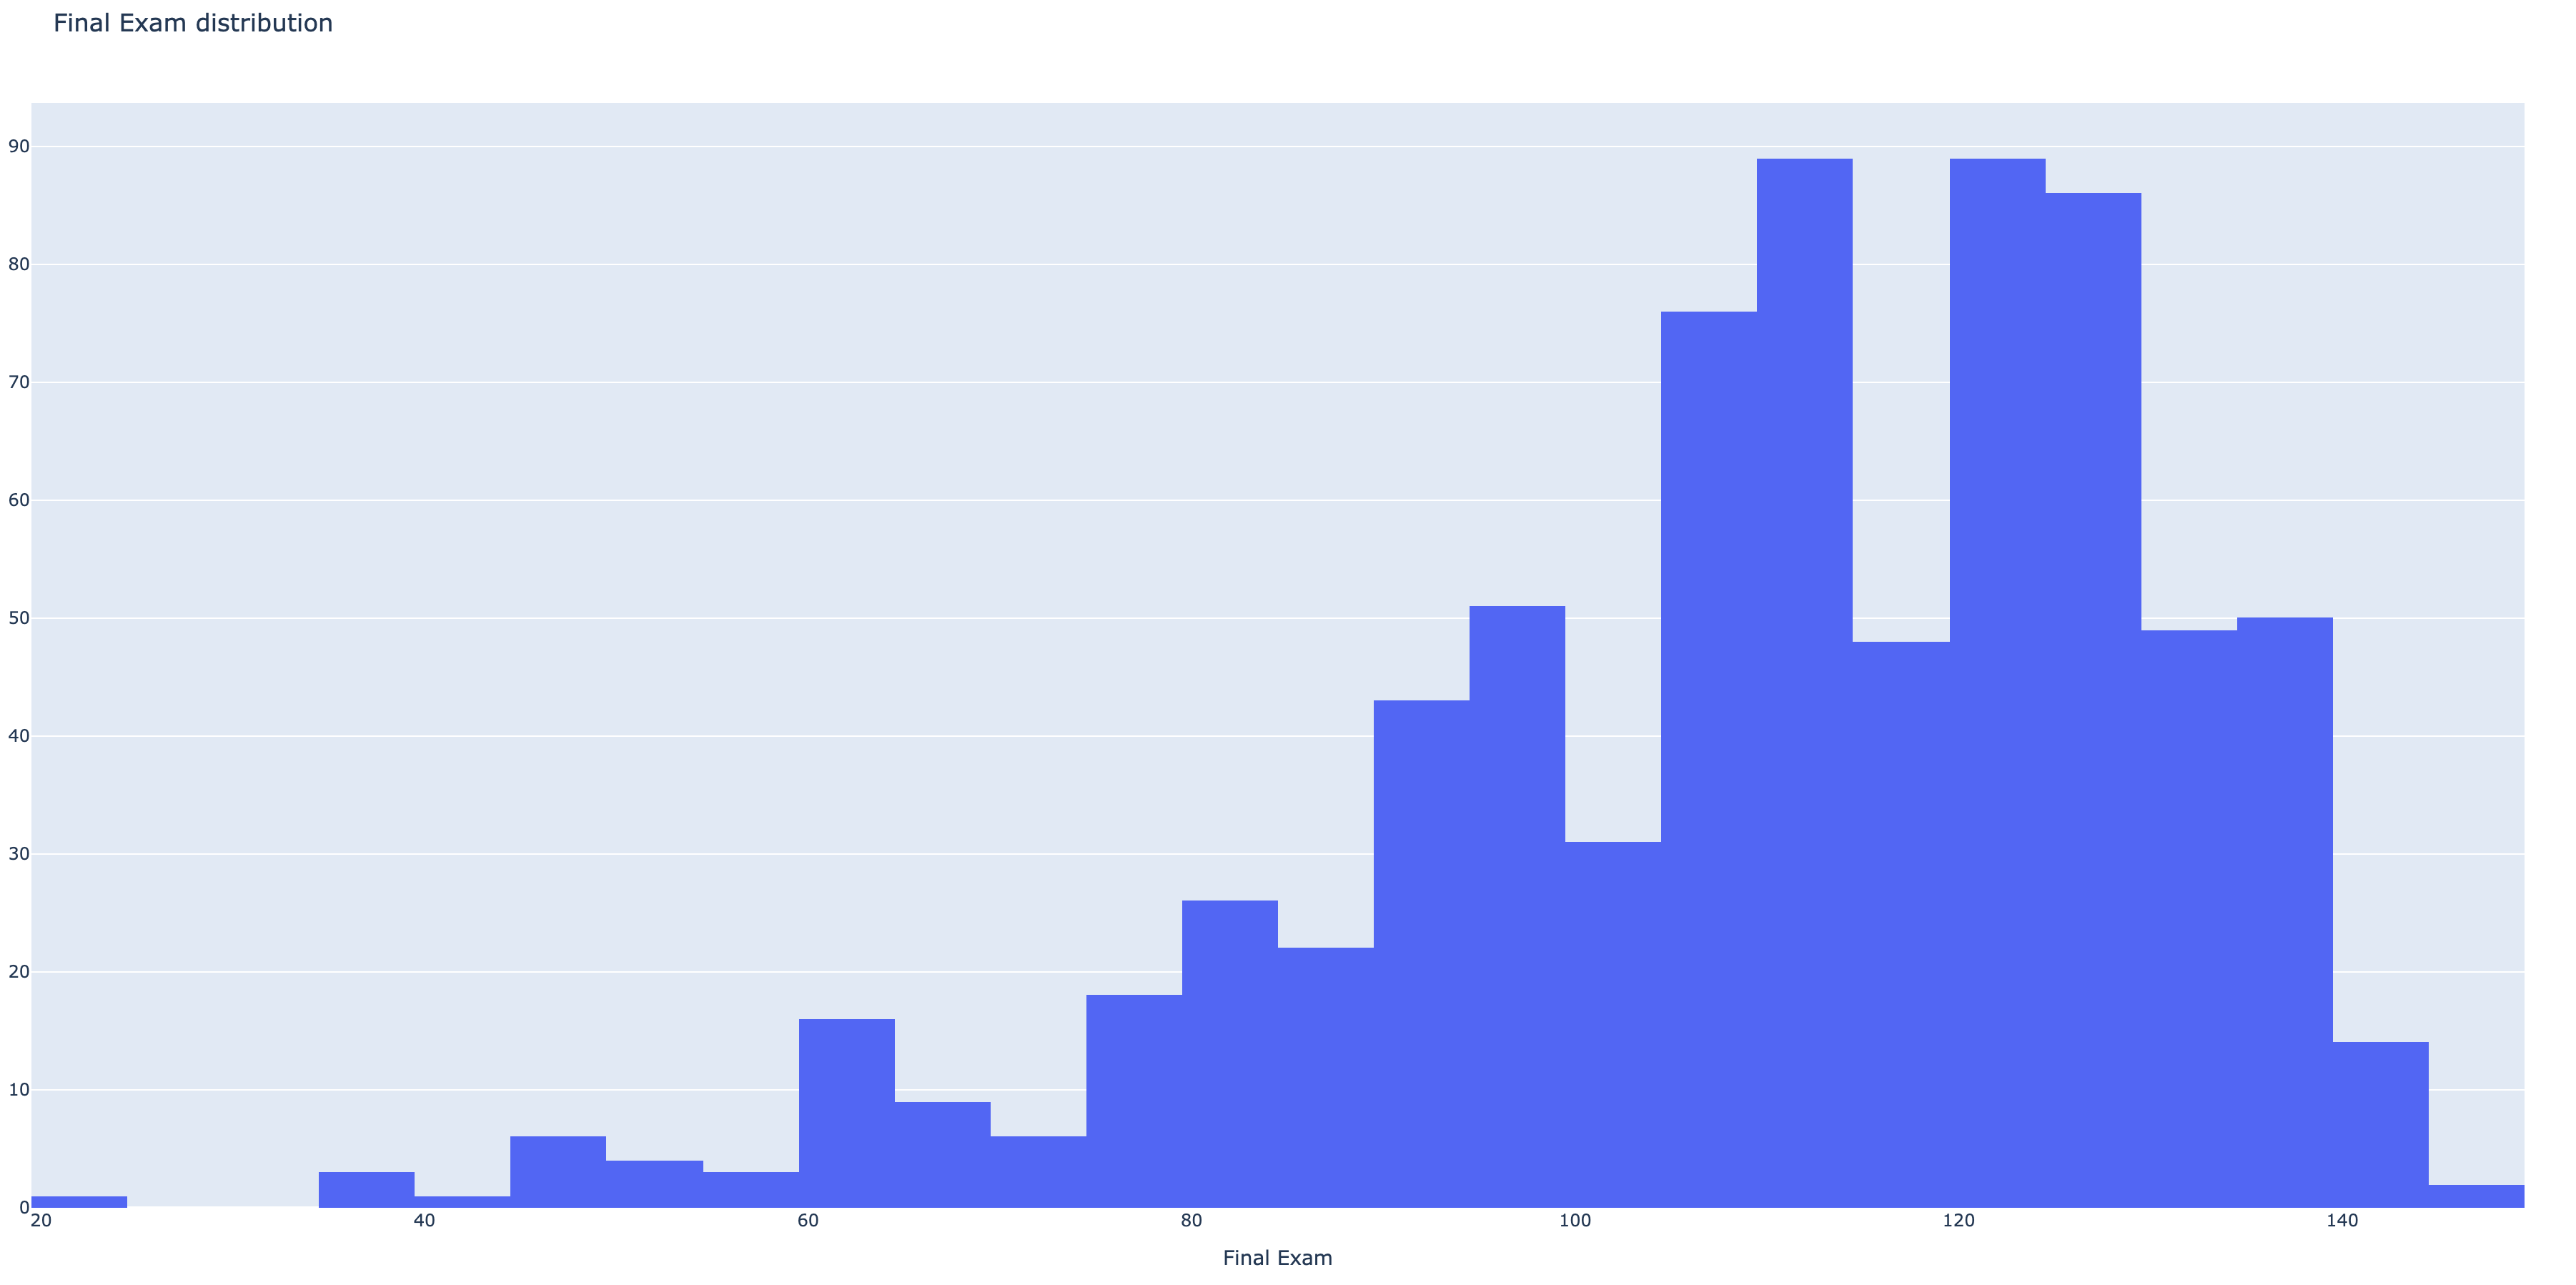
\includegraphics[width=15cm, height=8cm]{hist2.png}\\
This histogram shows the frequency distribution of the final exam scores for all students. From the graph we can see that the mast majority of scores received by students is around 110 and 130. There is also a bell-shaped distribution slightly right-skewed. This means that the majority of the students receive a decent score on this assignment.\\\\
6. Letter Grade histogram \\
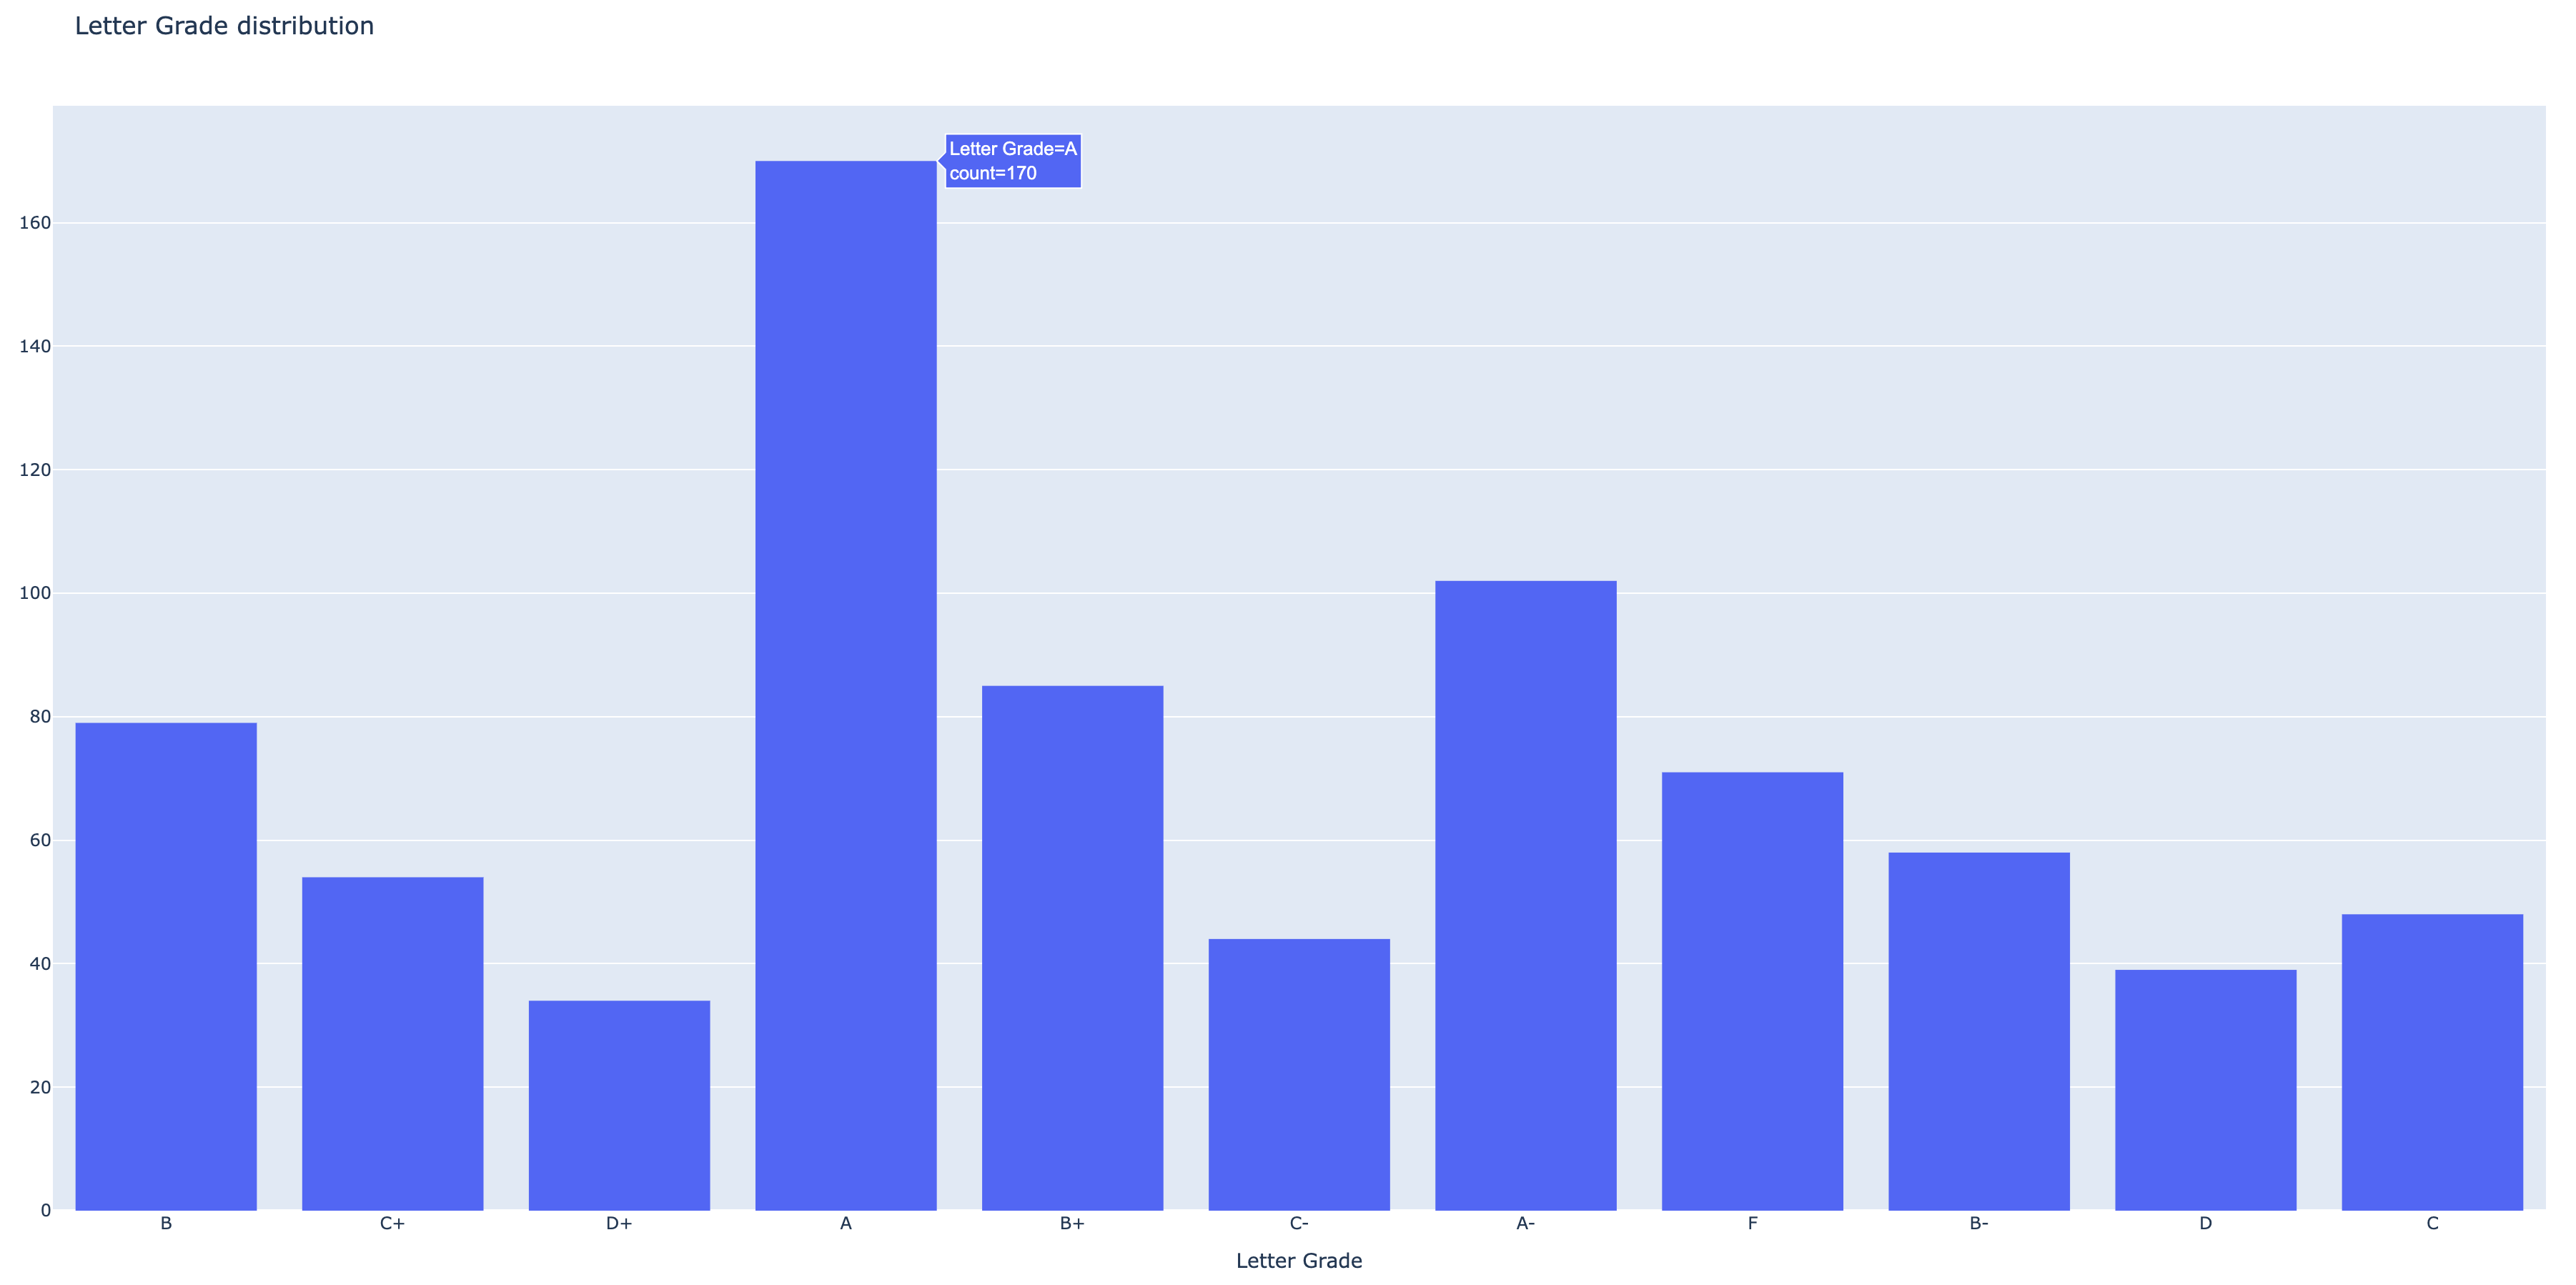
\includegraphics[width=15cm, height=8cm]{hist3.png}\\
This histogram shows the frequency distribution of the letter grades for all students. From the graph we can see that the majority of students ended up with an A for this course. However, one astonishing insight it shows is that there are more students who received F than students who received B-.\\\\
7. Peer Evaluations vs Total Score scatter plot \\
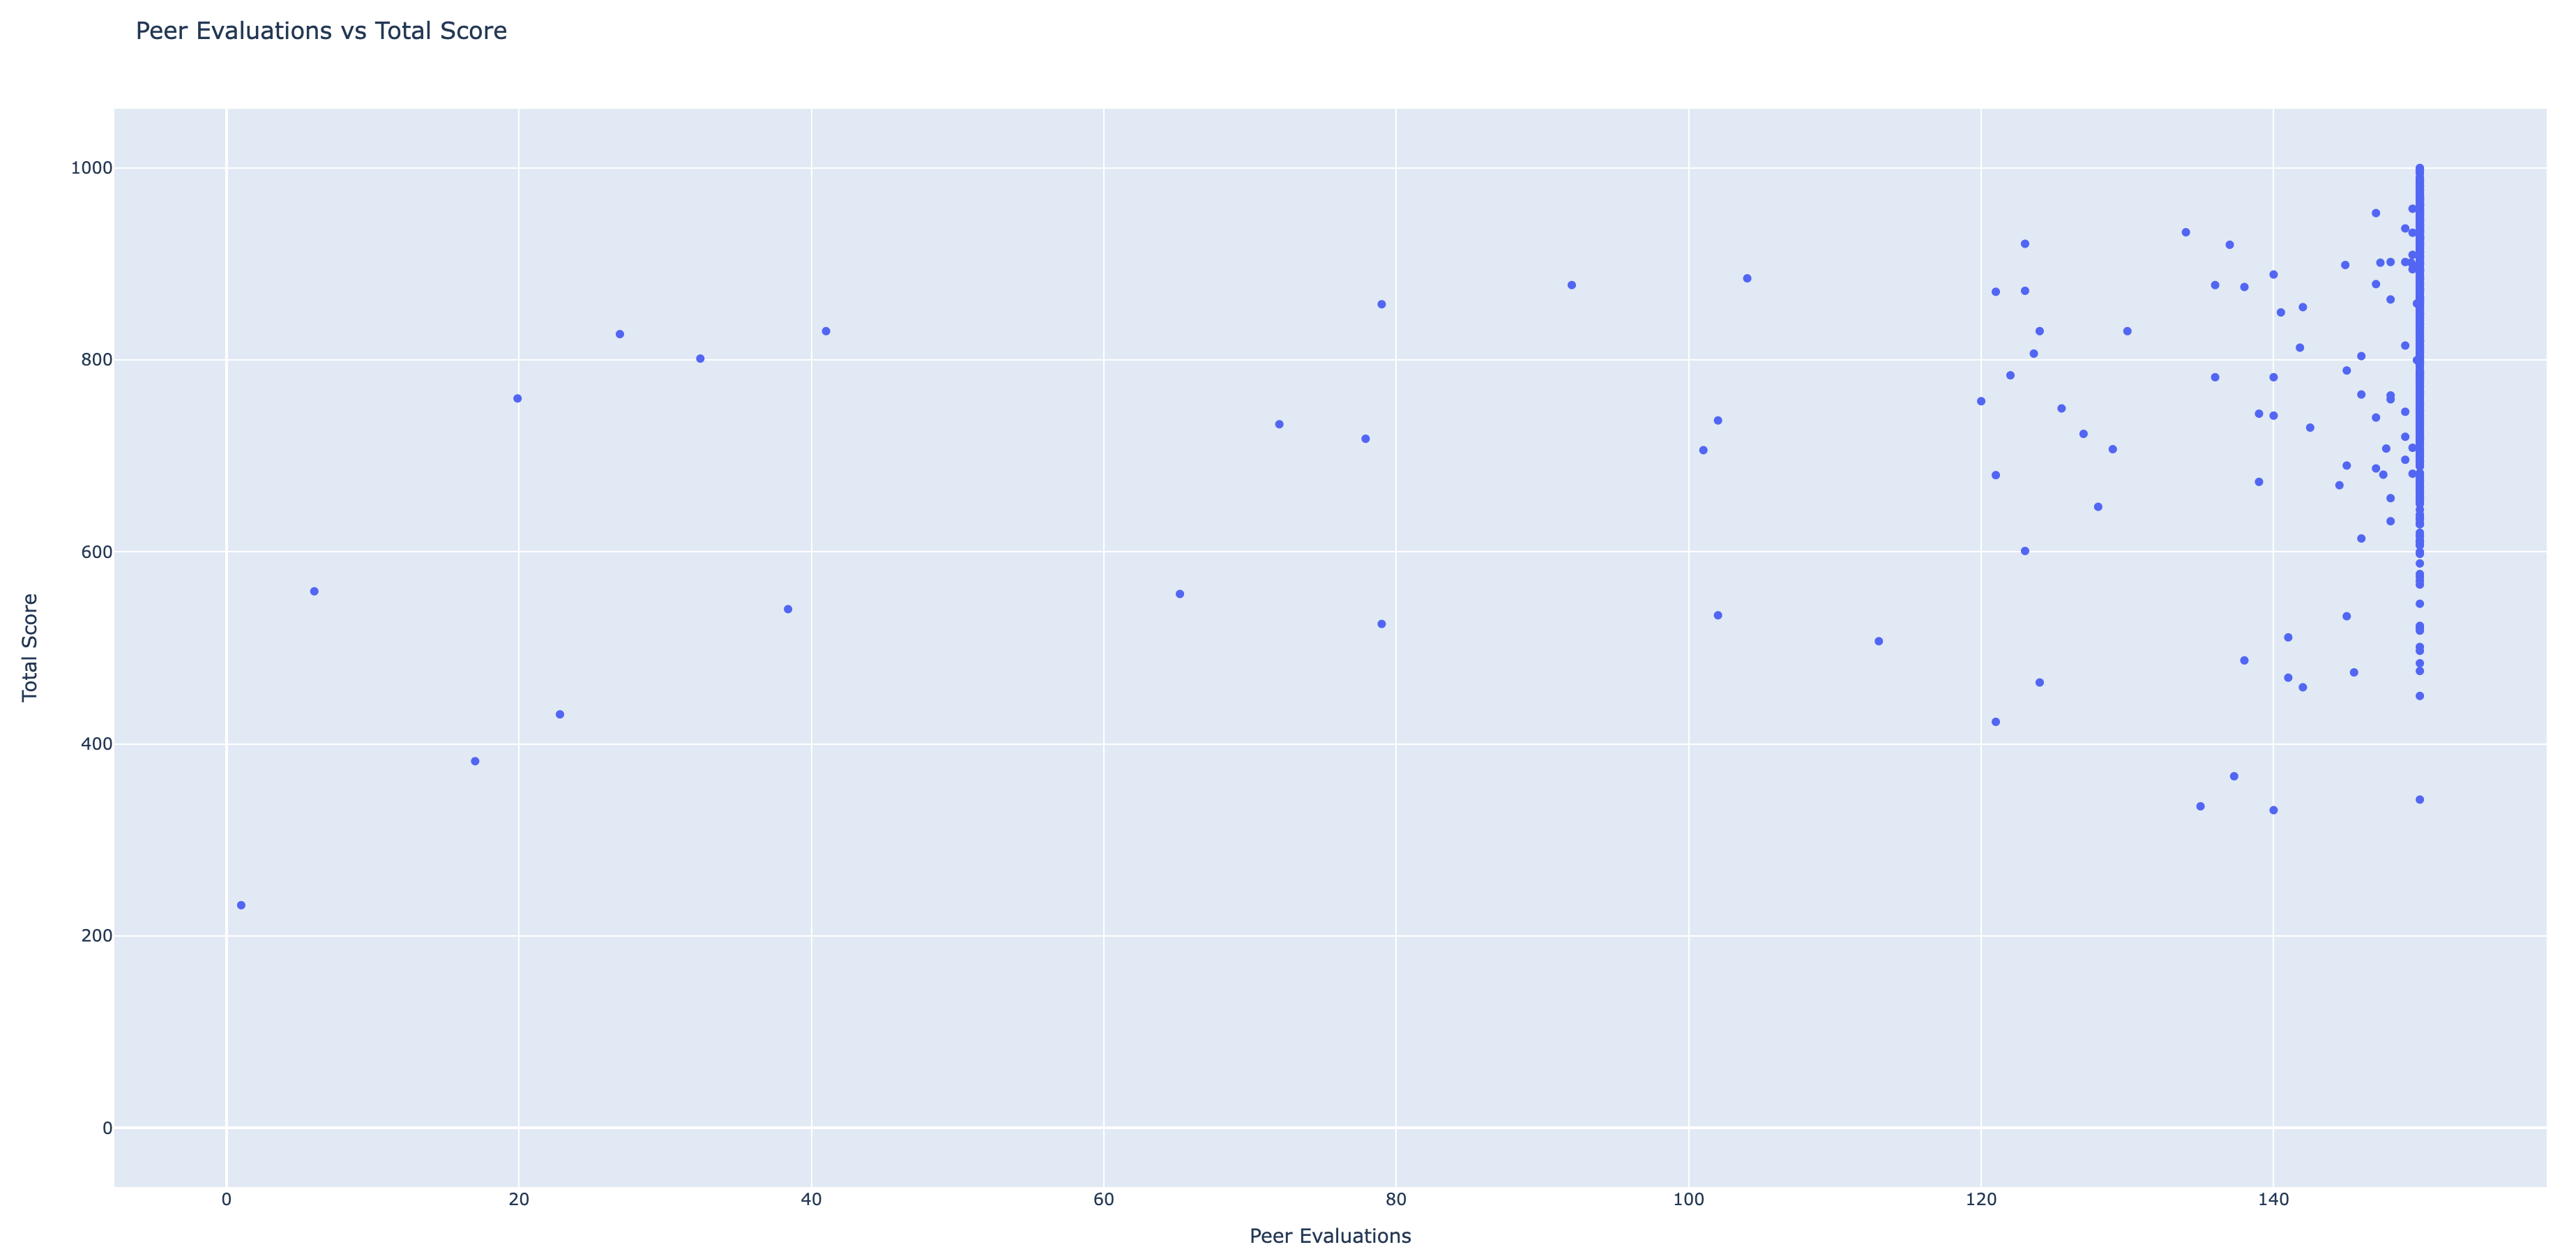
\includegraphics[width=15cm, height=8cm]{scatter1.png}\\
This scatter plot shows the distribution and relationship between a student's total score and peer evaluation score. From the graph, we can see that there is no obvious correlation between the two scores, as the overall trend is a flat line and people who received a full score on the peer evaluation could have both very high and very low total scores. \\\\
8. Final Exam vs Total Score scatter plot  \\
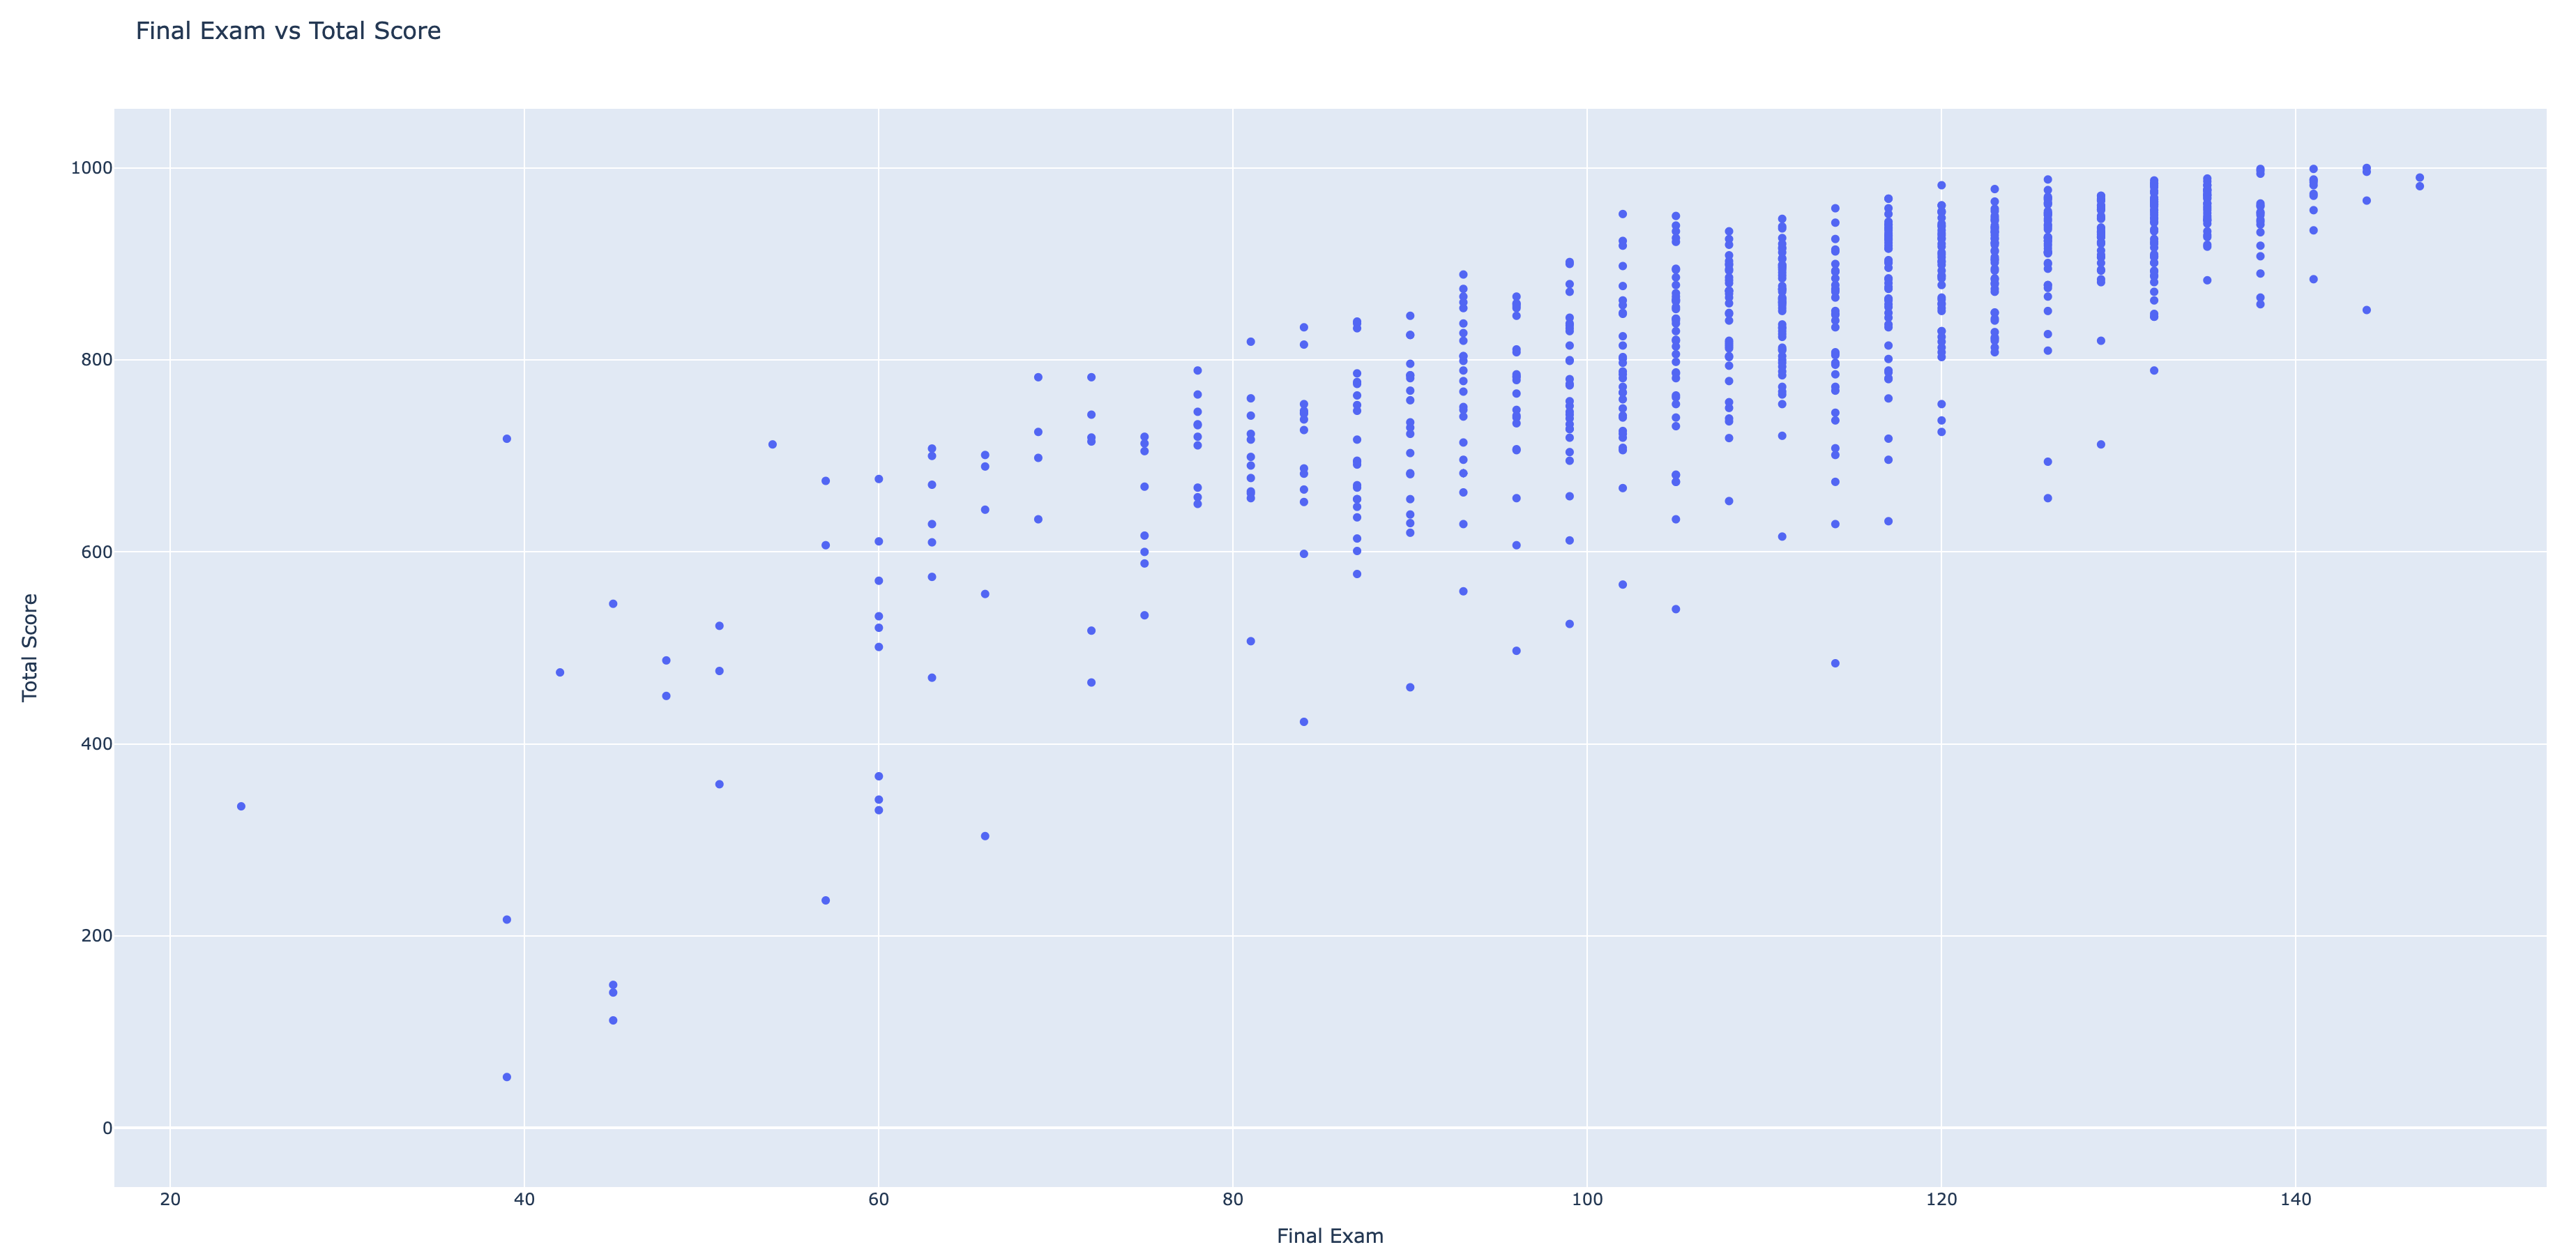
\includegraphics[width=15cm, height=8cm]{scatter2.png}\\
This scatter plot shows the distribution and relationship between a student's final exam score and total score. From the graph, we can see that there is a positive correlation between the two scores, as the overall trend is an increasing line and people who received a higher score on the final exam tend to have a higher total score. This makes sense because the final exam measures the student's overall ability and performance in the class, and it makes up a large portion of the total score. \\\\
9. Semester vs Total Score scatter plot \\
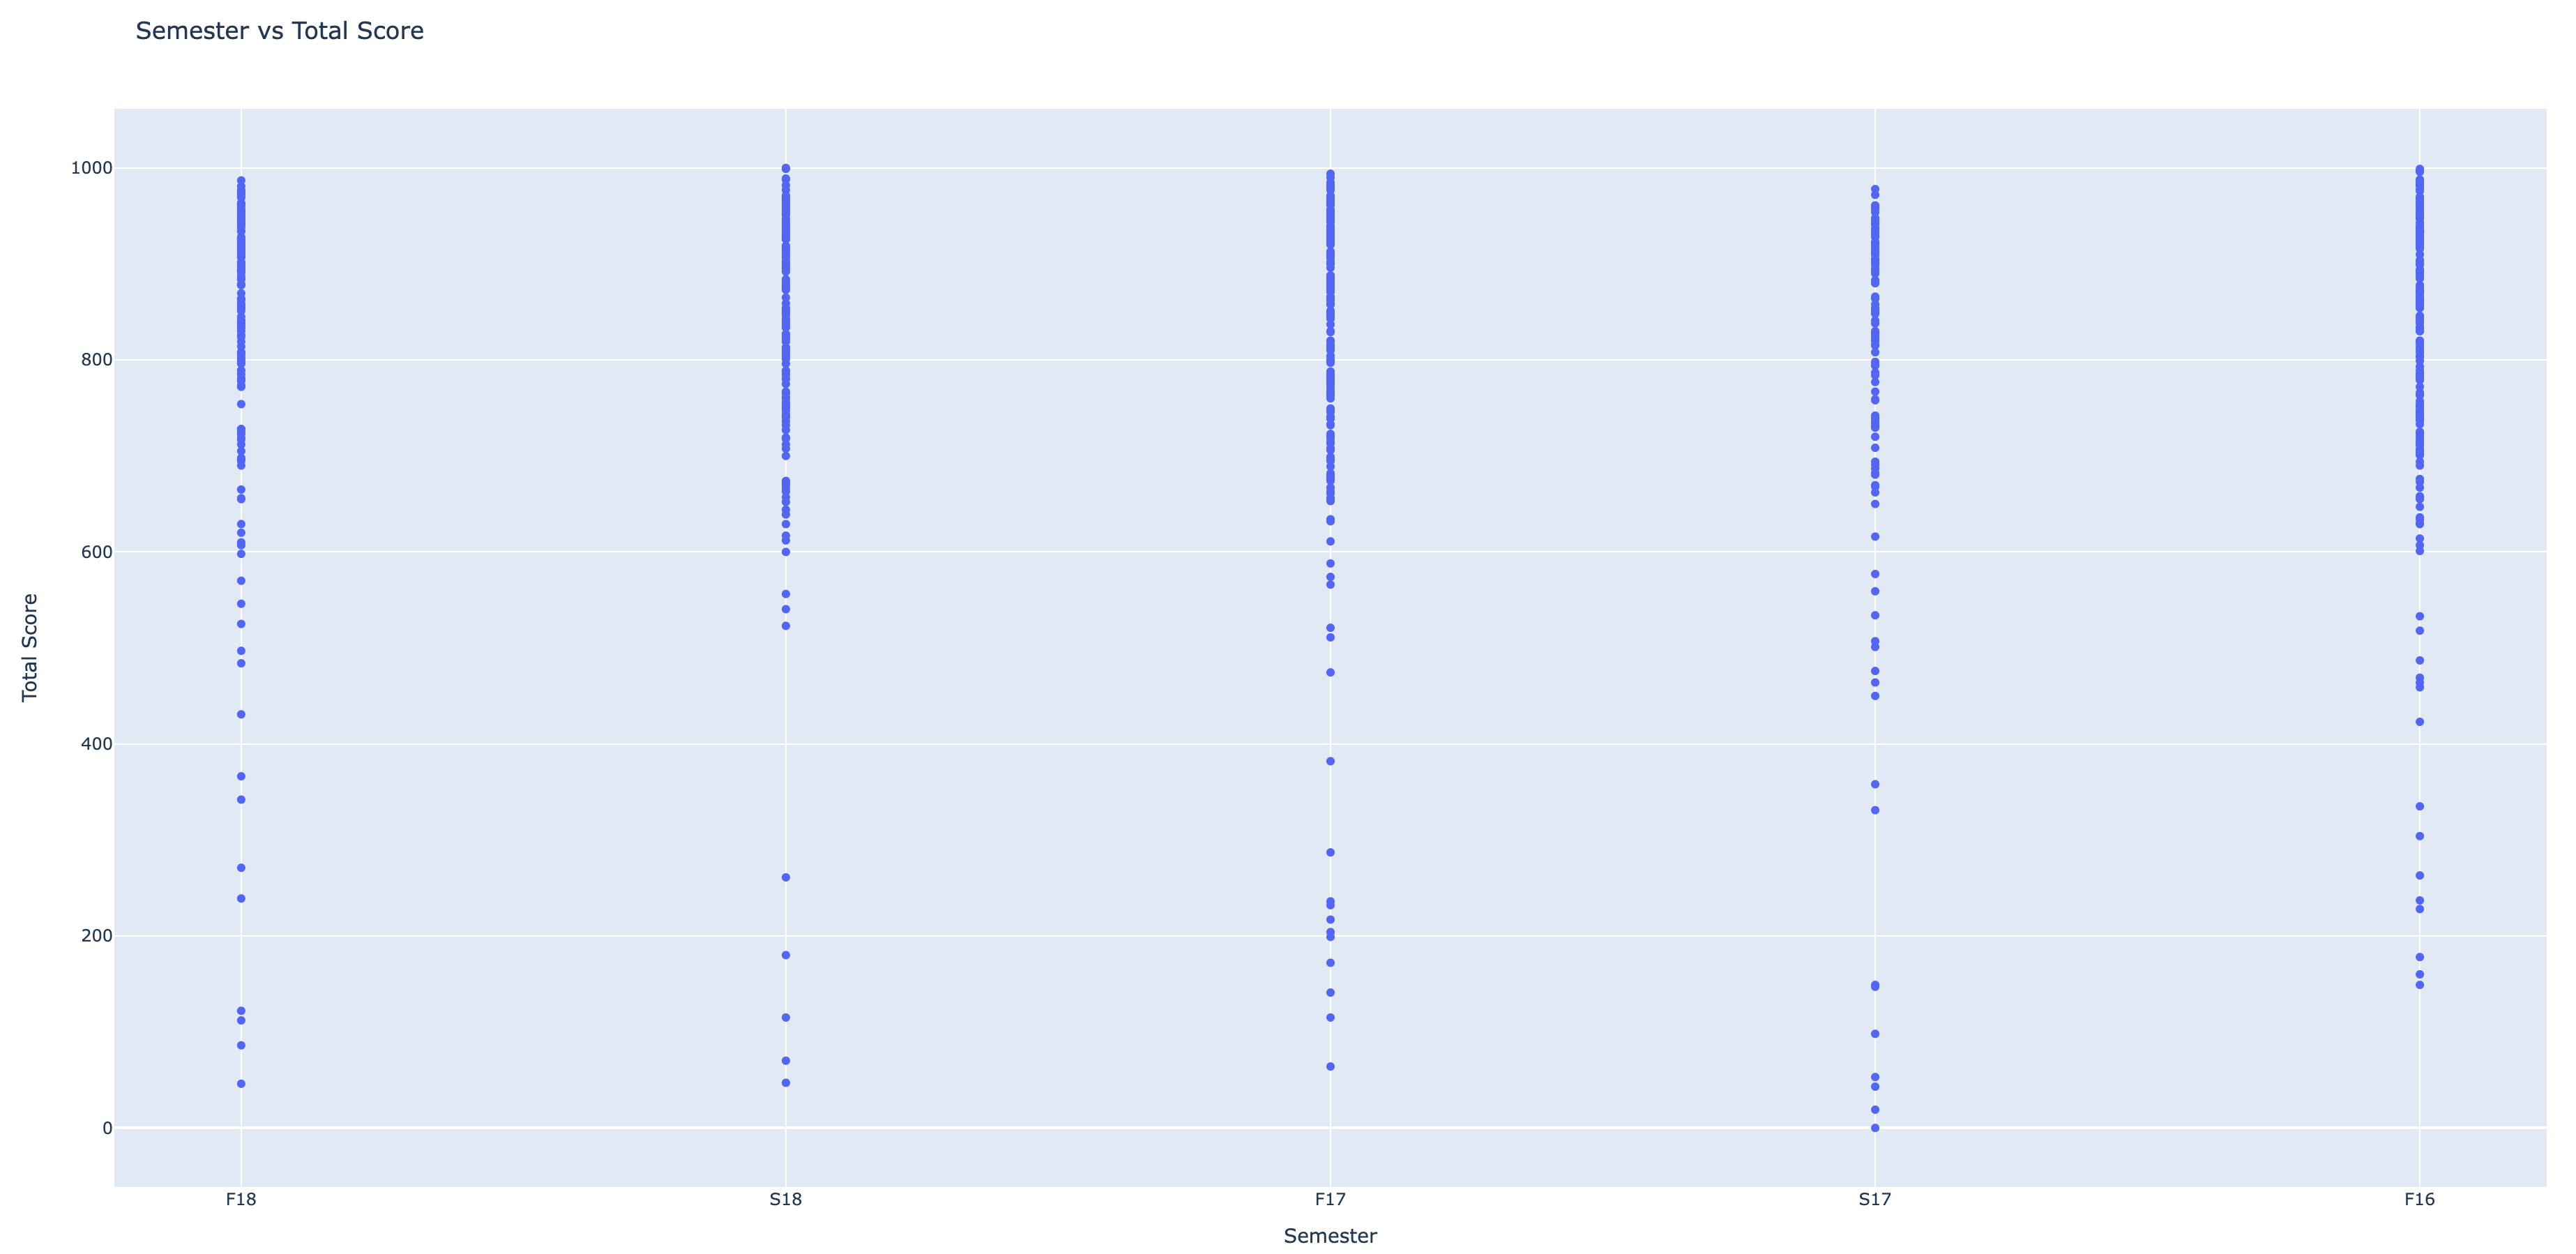
\includegraphics[width=15cm, height=8cm]{scatter3.png}\\
This scatter plot shows the distribution and relationship between semester and total scores. From the graph, we can see that different semesters have distinct total score distributions. For example, students from the fall of 2016 tend to be more consistent and are evenly distributed. There is no gap in the distribution and there are much fewer outliers. The next step would be to dive into that semester and see what makes it different from the rest and learn from the insights. \\\\
10. Average Total Score vs Semester \\
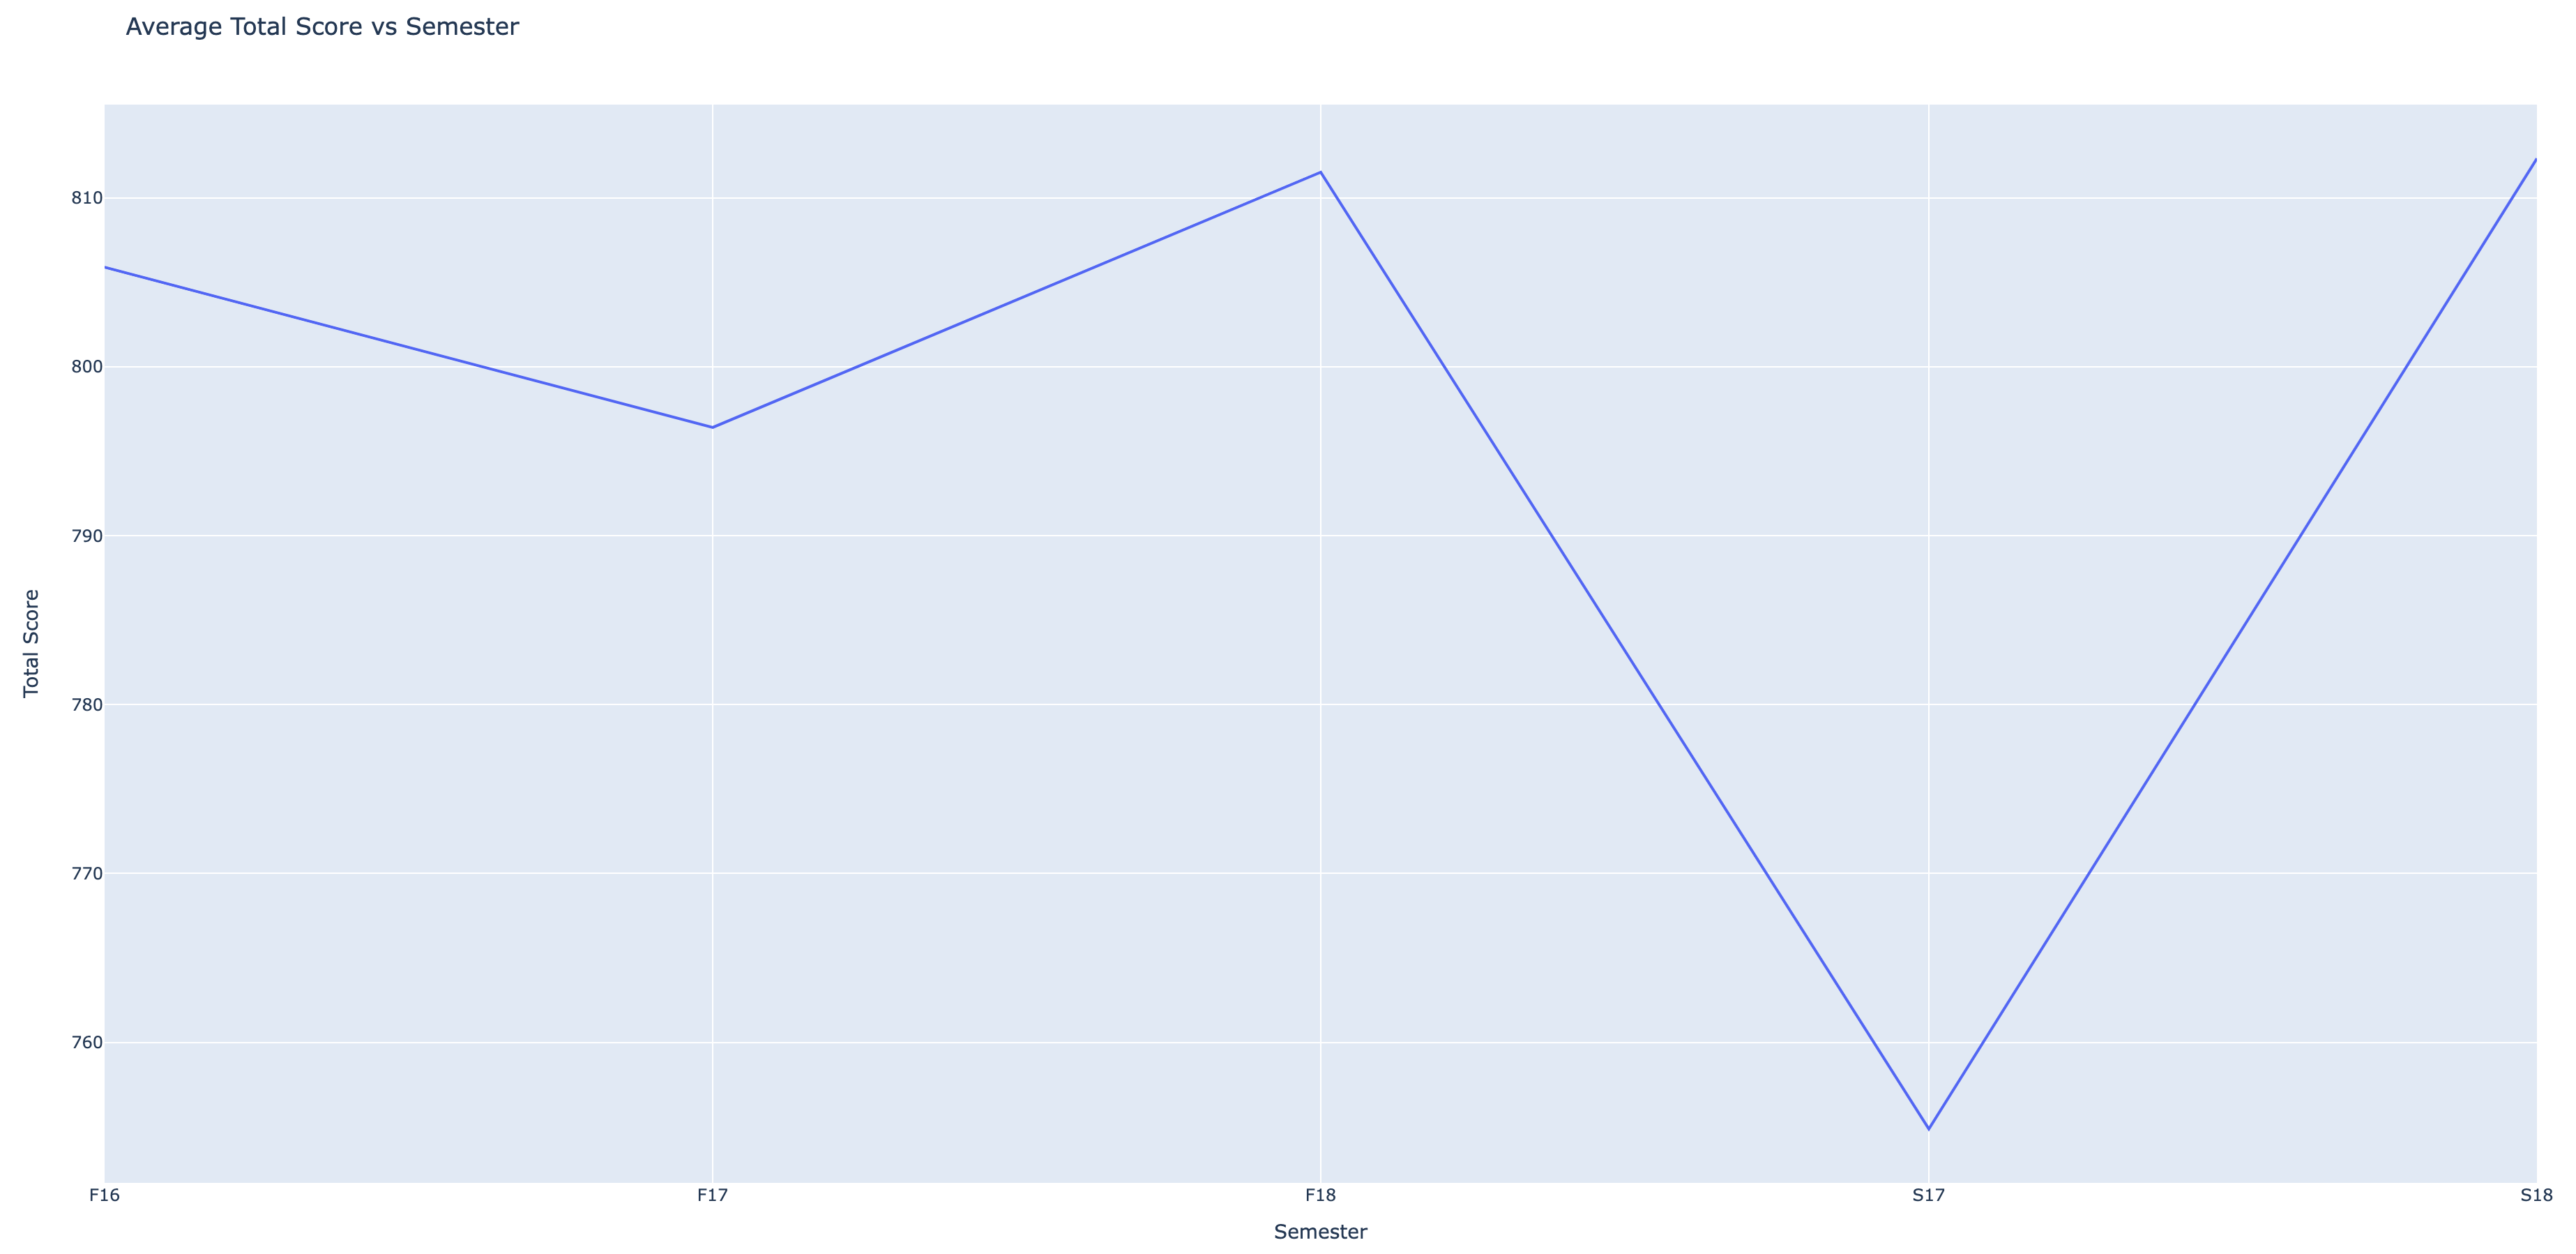
\includegraphics[width=15cm, height=8cm]{10.png}\\
This line plot shows how the average total score of all students in every semester changes. It is obvious that for the spring semester of 2017, the average score of students drops dramatically. This is problematic and we should compare other metrics of that semester to the rest in order to find out why exactly went wrong and prevent it from happening again. 


\section*{Problem 7 -  [Tools and languages]}
For this assignment, I used Python, specifically pandas data frame for the data manipulations and plotly for graphical analysis. I found Python extremely versatile and flexible, as I am able to create my own functions that simplify the computations for task 4. It is also well-documented, as I was able to find resources online where I can just learn how to perform certain operations. It is also very convenient when I tried to visualize my results. However, one thing that I noticed is that sometimes pandas data frame is different from SQL, with which I am more familiar from previous classes. This has caused me to do a lot of online searches to find the right syntax for the desired operations. 



\end{document}
